% =====================================================================
%  Praktikos ataskaita
%  IoT kibernetinių atakų prevencija naudojant DI sistemas
%
%  Kompiliavimas:  latexmk -pdf ataskaita.tex
%  arba rankiniu būdu:
%      pdflatex ataskaita → biber ataskaita → pdflatex ×2
% =====================================================================

\documentclass[12pt,a4paper]{article}

% ─── Koduotė ir kalba ────────────────────────────────────────────────
\usepackage[T1]{fontenc}
\usepackage[utf8]{inputenc}
\usepackage[lithuanian]{babel}     % lietuviški skyrių pavadinimai, kėlimas
\usepackage{lmodern}

% ─── Puslapio maketas ────────────────────────────────────────────────
\usepackage[a4paper,left=3cm,right=2cm,top=2.5cm,bottom=2.5cm]{geometry}
\usepackage{setspace}
\onehalfspacing
\usepackage{parskip}               % tarpai tarp pastraipų vietoj įtraukų

% ─── Lentelės ir grafika ─────────────────────────────────────────────
\usepackage{booktabs}              % \toprule \midrule \bottomrule
\usepackage{longtable}             % lentelės, netelpančios į puslapį
\usepackage{tabularx}
\usepackage{multirow}
\usepackage{siunitx}               % skaičių lygiavimas pagal kablelį
\sisetup{output-decimal-marker={,}, group-separator={\,}}
\usepackage{graphicx}
\graphicspath{{paveikslai/}}
\usepackage{float}
\usepackage{caption}
\captionsetup{font=small,labelfont=bf}

% ─── Kodas ───────────────────────────────────────────────────────────
\usepackage{listings}
\usepackage{xcolor}
\definecolor{kodofonas}{RGB}{248,248,248}
\lstset{
  basicstyle=\ttfamily\footnotesize,
  backgroundcolor=\color{kodofonas},
  frame=single,
  breaklines=true,
  numbers=left,
  numberstyle=\tiny\color{gray},
  captionpos=b,
  extendedchars=true,
  literate={ą}{{\k{a}}}1 {č}{{\v{c}}}1 {ę}{{\k{e}}}1 {ė}{{\.e}}1
           {į}{{\k{i}}}1 {š}{{\v{s}}}1 {ų}{{\k{u}}}1 {ū}{{\=u}}1 {ž}{{\v{z}}}1
}

% ─── Literatūra ──────────────────────────────────────────────────────
\usepackage{csquotes}
\usepackage[backend=biber,style=numeric,sorting=none,maxbibnames=99]{biblatex}
\addbibresource{saltiniai.bib}

% ─── Nuorodos (visada paskutinė) ─────────────────────────────────────
\usepackage[hidelinks]{hyperref}
\usepackage{cleveref}

% ─── Trumpiniai ──────────────────────────────────────────────────────
\newcommand{\lentele}[1]{\input{lenteles/#1}}

% =====================================================================
\begin{document}

% ─── Titulinis ───────────────────────────────────────────────────────
\begin{titlepage}
\centering
\vspace*{2cm}

{\large UNIVERSITETO PAVADINIMAS\\ FAKULTETO PAVADINIMAS\par}
\vspace{3cm}

{\Large\bfseries Vardas Pavardė\par}
\vspace{1.5cm}

{\huge\bfseries IoT kibernetinių atakų prevencija\\ naudojant dirbtinio intelekto sistemas\par}
\vspace{0.5cm}
{\Large Praktikos ataskaita\par}

\vfill
\begin{flushright}
Praktikos vadovas:\\ \textit{Vardas Pavardė}
\end{flushright}
\vspace{1cm}

{\large Vilnius, 2026\par}
\end{titlepage}

% ─── Turinys ─────────────────────────────────────────────────────────
\tableofcontents
\newpage

% ─── Skyriai ─────────────────────────────────────────────────────────
% Kol skyrius nebaigtas — užkomentuokite jį, kad kompiliuotųsi greičiau.

\section{Įvadas}
% =====================================================================
%  ĮVADAS — rašomas paskutinis (rugs. 18), bet failas reikalingas dabar,
%  kad ataskaita.tex kompiliuotųsi.
%  Tikslinė apimtis: 1–2 psl.
% =====================================================================

\subsection*{Temos aktualumas}

% TODO: IoT įrenginių skaičiaus augimas, jų silpna apsauga,
% Mirai tipo botnetų mastas. 2–3 pastraipos su nuorodomis.

\subsection*{Darbo tikslas}

Sukurti ir eksperimentiškai įvertinti dirbtiniu intelektu pagrįstą IoT tinklo
kibernetinių atakų aptikimo sprendimą.

\subsection*{Darbo uždaviniai}

\begin{enumerate}
  \item Išanalizuoti IoT tinklams būdingas kibernetines atakas ir jų aptikimo metodus.
  \item Išnagrinėti dirbtinio intelekto ir mašininio mokymosi metodų taikymo
        galimybes IoT tinklo atakoms aptikti.
  \item Parinkti ir pagrįsti tinkamus DI metodus IoT tinklo anomalijoms ir
        kibernetinėms atakoms identifikuoti.
  \item Sukurti DI pagrįstą IoT tinklo atakų aptikimo sprendimą.
  \item Eksperimentiškai įvertinti sukurto sprendimo tikslumą, klaidingų
        aptikimų skaičių ir kitus veikimo rodiklius.
  \item Palyginti skirtingų DI metodų efektyvumą aptinkant IoT tinklo atakas.
\end{enumerate}

\subsection*{Darbo struktūra}

% TODO (rugs. 18): 1 pastraipa — ką aprašo kiekvienas skyrius.


\section{IoT tinklų kibernetinės atakos ir jų aptikimo metodai}
\label{sec:atakos}
% =====================================================================
%  1 UŽDUOTIS — IoT tinklams būdingos kibernetinės atakos
%  Rugpjūčio 3–4 d. | Tikslinė apimtis: 4–5 psl.
% =====================================================================

\subsection{IoT architektūros sluoksniai ir jų atakų paviršius}

% TODO (rugpj. 3): trumpas trijų sluoksnių pristatymas (2 pastraipos)

\subsection{Atakų klasifikacija}

% TODO (rugpj. 3): po 1–2 pastraipas kiekvienam sluoksniui.
% Svarbiausia — stulpelis „matomi tinklo požymiai": jis tiesiogiai
% virsta modelio įvesties požymiais 4 skyriuje (\cref{sec:sprendimas}).

\begin{table}[H]
\centering
\caption{IoT atakų klasifikacija pagal architektūros sluoksnius}
\label{tab:atakos}
\small
\begin{tabularx}{\textwidth}{@{}l l X@{}}
\toprule
\textbf{Sluoksnis} & \textbf{Ataka} & \textbf{Matomi tinklo požymiai} \\
\midrule
Suvokimo & Jutiklių duomenų klastojimas & Netipinės telemetrijos reikšmės, staigūs šuoliai \\
         & Fizinis įsilaužimas & Naujas MAC adresas, pasikeitęs įrenginio profilis \\
\addlinespace
Tinklo   & DDoS / DoS & Didelis paketų dažnis, vienodas paketų dydis, daug SYN \\
         & MITM / ARP spoofing & Pasikartojantys ARP atsakymai, pasikeitęs maršrutas \\
         & Sybil & Daug tapatybių iš vieno fizinio šaltinio \\
         & RPL maršrutizavimo atakos & Anomalūs DIO/DAO pranešimai, topologijos kaita \\
\addlinespace
Programų & Mirai tipo botnetai & Telnet/SSH skenavimas, C\&C periodinės jungtys \\
         & MQTT piktnaudžiavimas & Netipiniai topic'ai, per didelis publish dažnis \\
         & Duomenų nutekinimas & Neįprastai didelis išeinantis srautas \\
\bottomrule
\end{tabularx}
\end{table}

\subsection{Klasikiniai aptikimo metodai ir jų ribos IoT kontekste}

% TODO (rugpj. 4): parašais grįstas (Snort/Suricata), taisyklėmis grįstas,
% anomalijomis grįstas — po pastraipą. Akcentas: KODĖL nepakanka.

\begin{table}[H]
\centering
\caption{Aptikimo metodų palyginimas IoT kontekste}
\label{tab:aptikimas}
\small
\begin{tabularx}{\textwidth}{@{}l X X@{}}
\toprule
\textbf{Metodas} & \textbf{Privalumai} & \textbf{Trūkumai IoT aplinkoje} \\
\midrule
Parašais grįstas & Tikslus žinomoms atakoms, mažai klaidingų teigiamų
& Neaptinka zero-day; parašų bazė reikalauja nuolatinio atnaujinimo \\
\addlinespace
Taisyklėmis / slenksčiais & Paprasta realizuoti, skaidru
& Daug klaidingų pavojaus signalų; slenksčiai netinka nevienalyčiam IoT elgesiui \\
\addlinespace
Anomalijomis grįstas & Aptinka nematytas atakas
& Reikia „normalaus elgesio" etalono; jautrus koncepcijos dreifui \\
\bottomrule
\end{tabularx}
\end{table}

\subsection{IoT specifika, ribojanti tradicinių IDS taikymą}

% TODO (rugpj. 4): riboti resursai, protokolų įvairovė, įrenginių mastas,
% nevienalytis normalaus elgesio profilis, šifruotas srautas.
% Ši dalis pagrindžia, kodėl 2 skyriuje kreipiamės į DI metodus.

\subsection{Aptikimo diegimo vieta}

% TODO (rugpj. 4): on-device / edge-gateway / cloud — privalumai ir trūkumai.
% Susieti su inferencijos delsos ir modelio dydžio matavimais 5 skyriuje.

\subsection{Skyriaus apibendrinimas}

% TODO: 1 pastraipa — kokie reikalavimai keliami aptikimo sprendimui.


\section{Dirbtinio intelekto metodų taikymas atakoms aptikti}
\label{sec:di_metodai}
% =====================================================================
%  2 UŽDUOTIS — DI ir mašininio mokymosi metodų taikymo galimybės
%  Rugsėjo 2 d. | Tikslinė apimtis: 5–6 psl. (RIBA 6,5)
%
%  REIKALINGA PREAMBULĖJE: \usepackage{xltabular}
%
%  Būklė: tab:metodai užpildyta (T3). Poskyrių tekstas — T2 medžiaga
%  faile rezultatai/darbiniai/metodu_apzvalga.md
% =====================================================================

\subsection{Vertinimo rėmas ir apžvalgos ašis}

Pirmame skyriuje iš IoT aplinkos savybių išvesti reikalavimai aptikimo
sprendimui (žr. \ref{tab:reikalavimai} lentelę). Šiame skyriuje jie
nekuriami iš naujo --- tik pritaikomi konkretiems metodams. Toks
paveldėjimas svarbus metodologiškai: kriterijai suformuluoti dar
nežinant, kurie metodai bus svarstomi, todėl atranka negali būti
pritempta prie iš anksto pageidaujamo atsakymo.

Metodai grupuojami pagal mokymosi paradigmą, o ne pagal algoritmų
šeimą. Tokį pasirinkimą lemia tai, kad metodo tinkamumą šiame darbe
labiausiai apibrėžia ne jo matematinė prigimtis, o tai, ko jis
reikalauja iš duomenų: pažymėtų pavyzdžių, sekos, tinklo topologijos ar
paskirstytų klientų. Tolesniuose poskyriuose matyti, kad būtent šis
reikalavimas dažniausiai ir nulemia, ar metodą apskritai galima
taikyti turimam duomenų rinkiniui.

\subsection{Prižiūrimas mokymasis}

Prižiūrimi metodai reikalauja pažymėtų mokymo pavyzdžių. Naudojamame
rinkinyje jų yra keliasdešimt milijonų, todėl paradigma taikytina be
išlygų, o jos riba yra kita: modelis atpažįsta tik tas atakas, kurių
pavyzdžių matė mokydamasis.

Lentelinei srauto statistikai atskaitos klasė yra sprendimų medžių
ansambliai. Jie skiriasi tuo, kaip derinami atskiri medžiai:
atsitiktinis miškas juos moko lygiagrečiai iš skirtingų imties poaibių
ir apjungia balsavimu, o gradientinio stiprinimo modeliai (XGBoost,
LightGBM) mokomi nuosekliai, kiekvienam taisant ankstesniųjų liekamąją
paklaidą. Abi kryptys tvarko klasių disbalansą svoriais, nedubliuodamos
duomenų, ir abi inferuoja per mikrosekundes
\cite{almahaqeri2026gradient}.

Kiti prižiūrimi metodai IoT kontekste susiduria su tuo pačiu
sunkumu --- jų kaina atsiduria ten, kur jos leisti negalima. Atraminių
vektorių mašinos mokymo sudėtingumas auga kvadratiškai ar kubiškai
imties atžvilgiu, o artimiausių kaimynų metodas mokymo fazės neturi,
tačiau kiekvienam sprendimui turi peržiūrėti visą mokymo aibę --- taigi
lėčiausias yra būtent tada, kai reikia atsakyti realiu laiku. Naivųjį
Bajeso klasifikatorių, pigiausią iš visų, atmeta jo paties prielaida:
požymių sąlyginis nepriklausomumas šiame rinkinyje paneigiamas
tiksliomis funkcinėmis priklausomybėmis tarp statistinių požymių.

\subsection{Neprižiūrimas mokymasis ir anomalijų aptikimas}

Neprižiūrimi metodai mokosi tik iš gerybinio srauto ir atakos pavyzdžių
nereikalauja. Tai vienintelė paradigma, iš principo galinti aptikti
nematytas grėsmes, todėl darbe, kurio objektas yra prevencija, ji
negali būti praleista. Naudojamame rinkinyje gerybinio srauto yra
daugiau nei milijonas įrašų --- mokymui su kaupu pakanka.

Autokoderis suspaudžia įvestį per siaurą sluoksnį ir mokosi ją atkurti;
neįprastas srautas atkuriamas prasčiau, todėl atkūrimo paklaida veikia
kaip anomalijos matas. Toks sprendimas realiame IoT sraute jau
demonstruotas visoje grandinėje nuo požymių išgavimo iki aptikimo
\cite{meidan2018nbaiot}. Izoliacijos miškas tą pačią užduotį sprendžia
kur kas pigiau: atsitiktiniai skaidymai anomalijas atskiria greičiau nei
tankiai išsidėsčiusius įprastus taškus. Vienos klasės atraminių vektorių
mašina koncepciškai artima, bet paveldi tą patį mokymo sudėtingumą kaip
ir prižiūrima jos atmaina. Klasterizavimo metodai duoda grupes, o ne
sprendimą, todėl tiesiogiai palyginti su kitais metodais jų nepavyktų.

Šiai paradigmai klasių disbalansas nėra taikytinas kriterijus. Modelis
mato tik gerybinį srautą, todėl santykiai tarp atakų klasių jo
mokymo nepasiekia --- tai ne pranašumas, o kitaip suformuluotas
uždavinys.

\subsection{Gilusis mokymasis}

Gilaus mokymosi patrauklumas grindžiamas gebėjimu pačiam išmokti
požymių reprezentaciją. Tačiau kiekviena architektūra tai daro
remdamasi prielaida apie duomenų sandarą, ir būtent čia paaiškėja
esminis šio darbo apribojimas: naudojamo rinkinio įrašas yra trisdešimt
šešios agreguotos statistikos, be eilės, be krypties ir be topologijos.

Konvoliuciniai tinklai remiasi prielaida, kad gretimos įvesties
reikšmės susijusios, tačiau požymių eilė lentelėje yra sutartinė.
Rekurentiniai tinklai ir dėmesio mechanizmu grįstos architektūros
modeliuoja seką, o rinkinyje nėra nei laiko žymos, nei eilės tarp
įrašų --- kiekvienas įrašas jau yra dešimties arba šimto paketų lango
apibendrinimas, taigi laiko matmuo į požymius jau suvyniotas. Grafų
neuroniniams tinklams reikia mazgų ir briaunų, o adresų ar krypties
rinkinyje nėra. Vienintelė architektūra, nedaranti nė vienos iš šių
prielaidų, yra daugiasluoksnis perceptronas; ribotų išteklių
įrenginiuose jis kartu su laikine konvoliucija rodo geriausią tikslumo
ir kainos santykį \cite{mazinani2026constrained}.

Iš to seka klausimas, kurį šis darbas ir tikrina: ar didesnis modelio
sudėtingumas duoda naudos, kai įvestis yra nedidelis skaičius
nepriklausomų statistikų.

\subsection{Paskirstytas mokymasis ir paaiškinamumas}

Federuotas mokymasis nėra atskiras algoritmas, o mokymo schema: modeliai
mokomi lokaliai, o centralizuojami tik jų svoriai, todėl srautas
nepalieka tinklo. IoT kontekste tai reikšminga privatumo požiūriu, o
ryšio kaina gali būti optimizuota \cite{nassef2026tinyml}. Schemai
reikia duomenų, padalytų į klientus pagal realų šaltinį; naudojamame
rinkinyje įrenginio identifikatoriaus nėra, todėl atsitiktinis
padalijimas imituotų vienodą pasiskirstymą ir tirtų ne tą reiškinį,
dėl kurio schema ir taikoma.

Paaiškinamumas nėra mokymosi paradigma, o skersinis sluoksnis. SHAP
metodas pateikia nuoseklias globalias ir lokalias požymių atributikas,
LIME --- greitesnius lokalius paaiškinimus pavieniams pranešimams
audituoti; abu reikalauja pastebimų skaičiavimo išteklių ir todėl
netinka realaus laiko grandinei \cite{mohale2025xai}. Dėl to šiame
darbe paaiškinamumas naudojamas kaip rezultatų analizės priemonė, o ne
kaip aptikimo sprendimo dalis. Ši skirtis atsispindi \ref{tab:metodai}
lentelės stulpelyje: savaime interpretuojami metodai sprendimą leidžia
parodyti be papildomos kainos, o ansambliams ir neuroniniams tinklams ta
pati galimybė pasiekiama tik atskiru skaičiavimu.


% =====================================================================
%  tab:metodai — metodų vertinimo matrica (T3)
% ---------------------------------------------------------------------
%  Kaip ir tab:atakos: xltabular NEGALI būti table float'e,
%  todėl \caption rašomas lentelės viduje.
%
%  Kiekvienas įvertinimas turi šaltinį arba žymą (aut.) — tuščių
%  langelių stulpelyje „Šalt.“ būti negali. Žr. plano 4 skyrių.
% =====================================================================

\begingroup
\footnotesize
\setlength{\tabcolsep}{3pt}
\sloppy
\begin{xltabular}{\textwidth}{@{}
  >{\raggedright\arraybackslash}p{2.8cm}
  >{\raggedright\arraybackslash}p{1.35cm}
  >{\centering\arraybackslash}p{1.0cm}
  >{\centering\arraybackslash}p{0.95cm}
  >{\centering\arraybackslash}p{1.05cm}
  >{\raggedright\arraybackslash}p{1.55cm}
  >{\raggedright\arraybackslash}X
  >{\raggedright\arraybackslash}p{1.7cm}@{}}
\caption{Dirbtinio intelekto metodų vertinimas pagal reikalavimus,
         kylančius iš IoT aplinkos savybių}
\label{tab:metodai} \\
\toprule
\textbf{Metodas} & \textbf{Para\-digma} & \textbf{Nemat. atakos}
  & \textbf{Moky\-mo kaina} & \textbf{Infe\-ren. kaina}
  & \textbf{Interpre\-tuojamumas} & \textbf{Atsparumas disbalansui}
  & \textbf{Šalt.} \\
\midrule
\endfirsthead
\multicolumn{8}{@{}l}{\itshape \ref{tab:metodai} lentelės tęsinys} \\
\toprule
\textbf{Metodas} & \textbf{Para\-digma} & \textbf{Nemat. atakos}
  & \textbf{Moky\-mo kaina} & \textbf{Infe\-ren. kaina}
  & \textbf{Interpre\-tuojamumas} & \textbf{Atsparumas disbalansui}
  & \textbf{Šalt.} \\
\midrule
\endhead
\bottomrule
\endlastfoot

% --- Prižiūrimas mokymasis ---
Sprendimų medis (CART) & Prižiūr. & Ne & maž. & maž. &
  savaiminis & silpnas; taisomas svoriais & (aut.) \\
Random Forest & Prižiūr. & Ne & vid. & maž. &
  per XAI & geras su \texttt{class\_weight} & \cite{imani2025imbalance} \\
XGBoost & Prižiūr. & Ne & vid. & maž. &
  per XAI & geras; \SI{1.05}{\micro\second} inferencija &
  \cite{almahaqeri2026gradient} \\
LightGBM & Prižiūr. & Ne & maž. & maž. &
  per XAI & geras; beveik lygu XGBoost & \cite{almahaqeri2026gradient} \\
SVM (RBF) & Prižiūr. & Ne & l. did. & vid. &
  juod. dėžė & vid.; $O(n^2)$--$O(n^3)$ mokymas & (aut.) \\
$k$ artimiausių kaimynų & Prižiūr. & Ne & --- & l. did. &
  savaiminis & prastas; kaimynystėje dominuoja gausios klasės &
  \cite{sallam2026gap} \\
Naive Bayes & Prižiūr. & Ne & maž. & maž. &
  savaiminis & vid.; prielaida pažeista & (aut.) \\
\addlinespace
% --- Neprižiūrimas mokymasis ---
Autokoderis & Neprižiūr. & \textbf{Taip} & vid. & maž. &
  juod. dėžė & neaktualus --- mokoma tik iš gerybinio srauto &
  \cite{meidan2018nbaiot} \\
Isolation Forest & Neprižiūr. & \textbf{Taip} & maž. & maž. &
  per XAI & neaktualus --- kaip ir autokoderio & (aut.) \\
One-Class SVM & Neprižiūr. & \textbf{Taip} & l. did. & vid. &
  juod. dėžė & neaktualus, bet mokymas netelpa & (aut.) \\
Klasterizavimas ($k$-vid., DBSCAN) & Neprižiūr. & Ribotai & vid. & vid. &
  per XAI & prastas; mažos grupės susilieja & (aut.) \\
\addlinespace
% --- Pusiau prižiūrimas ---
Savimoka (pseudo-žymėjimas) & Pusiau prižiūr. & Ne & vid. & maž. &
  kaip bazinio & \textbf{blogėja} --- pseudo-etiketės stiprina
  gausių klasių šališkumą & (aut.) \\
\addlinespace
% --- Gilusis mokymasis ---
Daugiasluoksnis perceptronas & Gilusis & Ne & vid. & maž. &
  juod. dėžė & vid.; svoriai nuostolio funkcijoje &
  \cite{mazinani2026constrained} \\
1D-CNN & Gilusis & Ne & did. & vid. &
  juod. dėžė & vid.; požymių eilė savavališka &
  \cite{mazinani2026constrained} \\
LSTM / GRU & Gilusis & Ne & did. & vid. &
  juod. dėžė & vid.; sekos duomenyse nėra &
  \cite{mazinani2026constrained} \\
Transformer & Gilusis & Ne & l. did. & did. &
  juod. dėžė & vid.; ta pati sekos problema & \cite{nassef2026tinyml} \\
Grafų neuroninis tinklas & Gilusis & Ribotai & l. did. & did. &
  juod. dėžė & vid.; \SIrange{120}{180}{\milli\second} Raspberry Pi 4 &
  \cite{nassef2026tinyml} \\
\addlinespace
% --- Paskirstytas mokymasis ---
Federuotas mokymasis (FedAvg)\textsuperscript{a} & Paskirst. & kaip bazinio &
  paskirst. & kaip bazinio & kaip bazinio &
  \textbf{blogėja} esant ne-IID duomenims & \cite{nassef2026tinyml} \\
\end{xltabular}

\vspace{-0.5em}
{\footnotesize
\textbf{Žymėjimai.} Kaina: \emph{maž.} — mažas, \emph{vid.} — vidutinis,
\emph{did.} — didelis, \emph{l.\ did.} — labai didelis;
„---“ reiškia, kad fazės nėra.
Interpretuojamumas: \emph{savaiminis} — sprendimą galima parodyti be
papildomų įrankių; \emph{per XAI} — reikia SHAP ar LIME, o tai
papildoma skaičiavimo kaina \cite{mohale2025xai};
\emph{juod.\ dėžė} — savaiminio paaiškinimo nėra.
Žyma \emph{(aut.)} nurodo, kad įvertinimas yra šio darbo autoriaus, o ne
perimtas iš šaltinio.
\textsuperscript{a}\,Federuotas mokymasis yra mokymo schema, o ne atskiras
algoritmas: jo savybės priklauso nuo bazinio modelio.
\par}
\endgroup

% ---------------------------------------------------------------------
% 2.6-2.9   (T5, T4, T6, T7)
% ---------------------------------------------------------------------
\subsection{Praktiniai apribojimai IoT aplinkoje}
\label{sec:apribojimai}

Ankstesniuose poskyriuose metodai vertinti pagal aptikimo galimybes.
Šis poskyris prideda antrą matmenį --- ar metodas apskritai gali veikti
ten, kur jį reikėtų įdiegti. Trys apribojimai yra kiekybiniai ir todėl
tinka kaip atrankos kriterijai: inferencijos delsa, mokymo kaina ir
klasių disbalansas.

\subsubsection{Inferencijos delsa ir diegimo vieta}

Pirmame skyriuje diegimo vieta pasirinkta kraštiniame šliuze, o jam
keliamas realaus laiko reikalavimas yra \SIrange{20}{50}{\milli\second}
vienam sprendimui; įrenginio lygmeniui skiriama
\SIrange{1}{10}{\milli\second}, debesiui ---
ne mažiau kaip \SI{100}{\milli\second} \cite{sallam2026gap}. Šie skaičiai leidžia
metodus vertinti ne abstrakčiai, o pagal tai, kiek biudžeto jie suvartoja.

Skirtumas tarp lentelinių ansamblių ir giliųjų architektūrų yra ne
laipsnio, o eilės. Gradientinio stiprinimo modelis tame pačiame
CICIoT2023 rinkinyje 34 klasių užduotyje inferuoja per
\SI{3.53}{\micro\second} vienam įrašui \cite{almahaqeri2026gradient} ---
tai \num{0.018}~\% griežtesniojo (\SI{20}{\milli\second}) biudžeto.
Hibridinis grafų ir rekurentinis modelis tame pačiame rinkinyje
reikalauja \SIrange{120}{180}{\milli\second} Raspberry~Pi~4 plokštėje
\cite{nassef2026tinyml}, t.\,y. nuo 2,4 iki 9 kartų \emph{daugiau} nei
leidžia biudžetas. Tarp šių dviejų verčių yra keturios eilės.

\begin{table}[htbp]
\centering
\caption{Metodų tinkamumas pagal diegimo vietos delsos biudžetą}
\label{tab:apribojimai}
\footnotesize
\setlength{\tabcolsep}{4pt}
\begin{tabularx}{\textwidth}{@{}
  >{\raggedright\arraybackslash}p{2.6cm}
  >{\raggedright\arraybackslash}p{2.0cm}
  >{\raggedright\arraybackslash}X
  >{\raggedright\arraybackslash}X@{}}
\toprule
\textbf{Diegimo vieta} & \textbf{Delsos biudžetas} & \textbf{Telpa}
  & \textbf{Netelpa} \\
\midrule
Įrenginys (mikro\-valdiklis) & \SIrange{1}{10}{\milli\second} &
  Kvantuotas MLP arba TCN (INT8, modelis mažesnis
  \textgreater\,90~\%) \cite{mazinani2026constrained} &
  Ansambliai --- ne dėl delsos, o dėl modelio dydžio atmintyje \\
\addlinespace
\textbf{Kraštinis šliuzas} & \SIrange{20}{50}{\milli\second} &
  XGBoost, LightGBM, Random Forest, Isolation Forest, MLP ---
  su kelių eilių atsarga &
  Hibridiniai gilieji modeliai
  (\SIrange{120}{180}{\milli\second}) \cite{nassef2026tinyml} \\
\addlinespace
Debesis & $\geq$~\SI{100}{\milli\second} & Visi apžvelgti metodai &
  Prarandamas reagavimas realiu laiku; srautas turi palikti tinklą \\
\bottomrule
\end{tabularx}
\end{table}

Skelbiamos vertės išmatuotos skirtinga aparatūra: mikrosekundinės ---
serverio klasės procesoriumi, \SIrange{120}{180}{\milli\second} ---
vienos plokštės kompiuteriu. Skirtumo eilė tai atlaiko:
\SI{3.53}{\micro\second} į \SI{20}{\milli\second} biudžetą telpa
\num{5669} kartus, todėl reikalavimą tenkintų ir tiek kartų lėtesnė
aparatūra.

Atskirai pažymėtina, kad neprižiūrimų metodų atveju skelbiamas dydis
dažnai yra ne inferencijos delsa, o \emph{aptikimo laikas}. Gilusis
autokoderis N-BaIoT rinkinyje ataką aptinka per
$174 \pm \SI{212}{\milli\second}$ \cite{meidan2018nbaiot}: šis dydis
apima ir srauto lango sukaupimą, ne vien modelio skaičiavimą.
Standartinis nuokrypis čia didesnis už vidurkį, todėl vien vidurkiu
remtis negalima. Todėl penktame skyriuje matuojama grynoji inferencijos delsa, o lango
sukaupimo laikas nurodomas atskirai.

\subsubsection{Mokymo kaina}

Mokymo kaina yra ne vienkartinis, o pasikartojantis dydis. Tinklo
elgsena kinta, todėl aptikimo modelis turi būti periodiškai
permokomas, o kraštinio šliuzo aplinkoje tam skiriama įprasta
aparatūra be grafinio spartintuvo. Dėl to mokymo sudėtingumas yra
atrankos kriterijus, o ne vien techninė aplinkybė.

Pirmiausia jis pašalina metodus, kurių mokymo sudėtingumas imties
atžvilgiu yra kvadratinis ar kubinis, --- atraminių vektorių mašiną ir
jos vienos klasės atmainą. Milijonų eilučių eilės imtyse toks
augimas mokymą paverčia nepraktišku nepriklausomai nuo turimos
aparatūros. Giliosioms architektūroms mokymo trukmė be spartintuvo
veikia kaip antras, nepriklausomas argumentas prie jau įvardyto
delsos perviršio.

\subsubsection{Klasių disbalansas}

Naudojamame rinkinyje disbalansas reiškiasi dviem skirtingais
santykiais, ir jie turi skirtingas pasekmes. Atakų ir gerybinio srauto
santykis yra $41{,}8:1$ --- dėl jo bendras tikslumas dvejetainėje
užduotyje tampa neinformatyvus, nes viską ataka žymintis modelis
pasiektų apie $97{,}7$~\%. Kur kas didesnis yra santykis tarp pačių
klasių: gausiausia klasė už rečiausią didesnė \num{5764} kartus.
Būtent antrasis santykis paaiškina, kodėl daugiaklasėje užduotyje
krinta makro vidurkiu skaičiuojamas F1 --- septynios klasės sudaro
mažiau nei $0{,}03$~\% duomenų ir kiekviena jų į makro vidurkį įeina
tokiu pat svoriu kaip milijoninės.

Tai patvirtina ir literatūra. Tame pačiame CICIoT2023 rinkinyje
gradientinio stiprinimo modelio tikslumas pereinant nuo dvejetainės
prie aštuonių klasių užduoties beveik nekinta ($99{,}61 \rightarrow
99{,}59$~\%), o makro-F1 krinta nuo $0{,}9952$ iki $0{,}8903$
\cite{almahaqeri2026gradient}. Tas pats modelis ir tie patys duomenys ---
skiriasi tik metrika ir užduoties detalumas.

Balansavimo priemonių palyginimas prie skirtingų disbalanso lygių rodo,
kad suderintas gradientinio stiprinimo modelis kartu su SMOTE metodu
duoda nuosekliai geriausią F1, o atsitiktinio miško tikslumas esant
stipriam disbalansui pastebimai krinta \cite{imani2025imbalance}. Tas
pats šaltinis pateikia ir metodinę pastabą, svarbią penktam skyriui:
didėjant disbalansui F1, Kappa ir Matthewso koreliacijos koeficientas
svyruoja stipriai, o ROC-AUC ir PR-AUC išlieka palyginti stabilūs.
Todėl šalia makro-F1 tikslinga pateikti ir PR-AUC.

\subsection{Susiję darbai ir skelbiami rezultatai}

Skelbiamų rezultatų apžvalga reikalinga ne tam, kad būtų surinkti aukšti
skaičiai, o tam, kad savo matavimams atsirastų atskaitos taškas.
\ref{tab:susije} lentelėje kiekvienam darbui nurodoma ne tik metrika,
bet ir užduoties detalumas bei tai, kas riboja rezultato aiškinimą.

Užduoties detalumo stulpelis yra būtinas, nes be jo skaičiai
nepalyginami. Tai geriausiai matyti to paties modelio eilutėse: tame
pačiame duomenų rinkinyje gradientinio stiprinimo modelio tikslumas
dvejetainėje ir aštuonių klasių užduotyse skiriasi vos šimtosiomis
procento dalimis, o makro vidurkiu skaičiuojamas F1 krinta nuo
$0{,}9952$ iki $0{,}8903$ \cite{almahaqeri2026gradient}. Darbas,
pateikiantis tik tikslumą ir nenurodantis klasių skaičiaus, tokio
skirtumo neatskleidžia.

Antra pastebima savybė --- ne visos abejonės kyla dėl silpnų metrikų.
Dalis darbų skelbia aukštus F1 įverčius, tačiau užduoties detalumo
nenurodo \cite{nassef2026tinyml}, kitas pateikia suminį kompromiso
įvertį vietoj metrikų kiekvienam modeliui \cite{mazinani2026constrained},
o klasikiniame botnetų aptikimo darbe pasiektas šimtaprocentinis
teisingai atpažintų atakų dažnis atitinka lengviausią įmanomą
formuluotę --- atskiras modelis kiekvienam įrenginiui ir dvi botnetų
šeimos \cite{meidan2018nbaiot}. Trūkstamas metodikos elementas riboja
palyginimą lygiai taip pat, kaip ir prastas rezultatas.

Sugretinant savo rezultatus su šiais darbais svarbu turėti omenyje
požymių aibės skirtumą. Dauguma publikacijų remiasi pilna keturiasdešimt
šešių požymių versija, o šiame darbe naudojamame leidime jų
trisdešimt devyni: pašalinti krypties požymiai ir iš jų išvestos
statistikos. Dalis literatūroje aukštai reitinguojamų požymių šiame
leidime neegzistuoja, todėl skelbiami įverčiai laikytini bendru
atskaitos lygiu, o ne tiesioginiu palyginimo tašku. Į tai atsižvelgiama
šeštame skyriuje.

Iš apžvalgos taip pat matyti, kokio dydžio rezultato realu tikėtis.
Aštuonių kategorijų užduotyje geriausias literatūroje skelbiamas makro-F1
yra apie $0{,}89$; tai ir yra vertė, prie kurios lyginami šio darbo
matavimai --- ne artimi vienetui tikslumo įverčiai, gaunami dvejetainėje
formuluotėje.

% =====================================================================
%  tab:susije -- susije darbai ir skelbiami rezultatai (T4)
% ---------------------------------------------------------------------
%  Stulpelis "Uzduotis" yra butinas: be jo metrikos nepalyginamos.
%  Stulpelis "Kas kelia abejoniu" yra visa lenteles verte -- be jo
%  tai citatu sarasas, ne analize.
%
%  BUKLE 2026-09-02: 8 eilutes is 3 saltiniu -- visi skaiciai patikrinti
%  leidejo puslapyje. TRUKSTA 4 eiluciu (zr. komentara po lentele).
% =====================================================================

\begingroup
\footnotesize
\setlength{\tabcolsep}{3pt}
\sloppy
\begin{xltabular}{\textwidth}{@{}
  >{\raggedright\arraybackslash}p{2.0cm}
  >{\raggedright\arraybackslash}p{2.0cm}
  >{\raggedright\arraybackslash}p{2.1cm}
  >{\raggedright\arraybackslash}p{1.5cm}
  >{\raggedright\arraybackslash}p{2.8cm}
  >{\raggedright\arraybackslash}X@{}}
\caption{Skelbiami dirbtinio intelekto metodų rezultatai IoT įsibrovimų
         aptikimo darbuose}
\label{tab:susije} \\
\toprule
\textbf{Šaltinis} & \textbf{Duomenų rinkinys} & \textbf{Metodas}
  & \textbf{Užduotis} & \textbf{Skelbiama metrika}
  & \textbf{Kas kelia abejonių} \\
\midrule
\endfirsthead
\multicolumn{6}{@{}l}{\itshape \ref{tab:susije} lentelės tęsinys} \\
\toprule
\textbf{Šaltinis} & \textbf{Duomenų rinkinys} & \textbf{Metodas}
  & \textbf{Užduotis} & \textbf{Skelbiama metrika}
  & \textbf{Kas kelia abejonių} \\
\midrule
\endhead
\bottomrule
\endlastfoot

\cite{almahaqeri2026gradient} & CICIoT2023 (46 pož.) & XGBoost &
  dvejetainė & tikslumas 99,61~\%; macro-F1 0,9952;
  \SI{0.36}{\micro\second}/įrašui &
  Naudota pilna 46 požymių aibė; šio darbo leidime jų 39 \\
\cite{almahaqeri2026gradient} & CICIoT2023 (46 pož.) & XGBoost &
  8 klasės & tikslumas 99,59~\%; \textbf{macro-F1 0,8903};
  \SI{1.05}{\micro\second} &
  Tikslumas beveik nepakito, o macro-F1 krito 0,10 --- tas pats modelis,
  tie patys duomenys \\
\cite{almahaqeri2026gradient} & CICIoT2023 (46 pož.) & XGBoost &
  34 klasės & tikslumas 99,48~\%; macro-F1 0,8876;
  \SI{3.53}{\micro\second} &
  Tas pats dėsningumas ryškėja dar labiau \\
\cite{almahaqeri2026gradient} & CICIoT2023 (46 pož.) & LightGBM &
  dvejetainė & tikslumas 99,53~\%; macro-F1 0,9944;
  \SI{0.72}{\micro\second} &
  Skirtumas nuo XGBoost mažesnis nei tikėtinas matavimo svyravimas \\
\addlinespace
\cite{nassef2026tinyml} & CICIoT2023 & GAT + BiGRU, federuotas
  mokymasis & nenurodyta & F1 0,92; \SIrange{120}{180}{\milli\second}
  Raspberry Pi 4 &
  Užduoties granuliarumas nenurodytas; delsa 2,4--9 kartų viršija
  \SIrange{20}{50}{\milli\second} šliuzo biudžetą \cite{sallam2026gap} \\
\cite{nassef2026tinyml} & Edge-IIoTset & GAT + BiGRU &
  nenurodyta & F1 0,94 &
  Ta pati problema; pramoninis rinkinys, kitas įrenginių profilis \\
\cite{nassef2026tinyml} & RT-IoT2022 & GAT + BiGRU &
  nenurodyta & F1 0,93 &
  Ta pati problema \\
\addlinespace
\cite{mazinani2026constrained} & CICIoT2023 (46,7~mln. įrašų) &
  MLP, TCN, CNN, LSTM, GRU, SimpleRNN & dvejetainė, 8 ir 34 klasės &
  MLP ir TCN --- geriausias tikslumo ir kainos kompromisas;
  INT8 kvantavimas mažina modelį \textgreater\,90~\% &
  Skelbiamas suminis kompromiso balas, o ne metrikos kiekvienam
  modeliui, todėl tiesiogiai palyginti neįmanoma \\
\addlinespace
\cite{meidan2018nbaiot} & N-BaIoT (9 įrenginiai) & gilusis
  autokoderis & dvejetainė, kiekvienam įrenginiui atskirai &
  TPR 100~\%; FPR $0{,}007 \pm 0{,}01$; aptikimo laikas
  $174 \pm \SI{212}{\milli\second}$ &
  TPR 100~\% pasiektas lengviausioje įmanomoje formuluotėje ---
  vienas įrenginys, dvi botnetų šeimos; aptikimo laiko standartinis
  nuokrypis didesnis už vidurkį \\
\addlinespace
\cite{eren2026drift} & BoT-IoT, ToN-IoT, UNSW-NB15 & įvairūs
  klasifikatoriai & kryžminis perkėlimas &
  vidutinis MCC krinta nuo ${\sim}94~\%$ iki ${\sim}29~\%$ &
  Viename rinkinyje gauti skaičiai kitame negalioja \\
\end{xltabular}
\endgroup

% ---------------------------------------------------------------------
%  BUKLE 2026-09-02, 15:10: uzpildyta 10 eiluciu is 5 saltiniu.
%
%  LIEKA 1 EILUTE:
%   houichi2025smartcity -- CICIoT2023, klasikiniai MM metodai.
%     Leidejo puslapis grazina 403, ResearchGate 429. Reikia
%     universiteto prieigos. Uzpildyti: metodas, uzduotis, metrika.
%
%  NEIEJO I LENTELE (sazininga pataisa):
%   imani2025imbalance -- naudoja telekomunikaciju klientu nutekejimo
%     duomenis su dirbtinai nustatytais disbalanso lygiais (15/10/5/1 %),
%     NE IoT idsibrovimu rinkini. Todel tai NE susijes darbas, o
%     metodologinis saltinis -> 2.6 poskyris (balansavimo pasirinkimas).
% ---------------------------------------------------------------------
% ---------------------------------------------------------------------
% 2.8 ATSISAKYTA (2026-09-02): "galiojimo ribos be kryzminio
%   patikrinimo" isbraukta. Priezastis - vieta, ne apimtis: 2 skyrius
%   apzvelgia metodus, o rezultatu galiojimo ribos priklauso
%   metodikai (4 sk.) ir apribojimu aptarimui (6 sk.). Antriniu
%   rinkiniu tiesiog nera - to konstatavimas nereikalauja poskyrio.
%   Perkelta: viena pastraipa i 4 sk. metodika (skaidymo sprendimas).
\subsection{Skyriaus apibendrinimas: kandidatų aibė}
\label{sec:kandidatai}

Apžvelgti aštuoniolika metodų (žr. \ref{tab:metodai} lentelę).
Kandidatų aibę labiausiai siaurina naudojamų duomenų sandara. Galutinę
atranką su kriterijų svoriais atlieka trečias skyrius; čia fiksuojama,
iš ko renkamasi.

\subsubsection{Keturi pasirinkti metodai}

\textbf{Atsitiktinis miškas} imamas kaip atskaitos modelis. Jis
nereikalauja kruopštaus derinimo, atsparus persimokymui, o klasių svoriai
leidžia tvarkyti disbalansą nedubliuojant duomenų. Jis nustato
atskaitos lygį, prie kurio matuojamas sudėtingesnių metodų duodamas
prieaugis.

\textbf{Gradientinio stiprinimo modelis} (XGBoost) yra laukiamas
geriausias prižiūrimas metodas: tame pačiame duomenų rinkinyje jis
pranoko dešimt kitų metodų, o inferencijos trukmė matuojama
mikrosekundėmis \cite{almahaqeri2026gradient}. Kartu jis yra vienintelis
tiesiogiai palyginamas atskaitos taškas literatūroje.

\textbf{Daugiasluoksnis perceptronas} įtraukiamas kaip vienintelė gilaus
mokymosi architektūra, prasminga lentelinei įvesčiai --- ji nedaro
prielaidų nei apie požymių eilę, nei apie kaimynystę, nei apie seką.
Ribotų išteklių įrenginiuose jis kartu su laikine konvoliucija rodo
geriausią tikslumo ir kainos santykį \cite{mazinani2026constrained}.
Jo paskirtis --- patikrinti, ar didesnis modelio sudėtingumas duoda
naudos ten, kur įvestis yra trisdešimt šešios nepriklausomos
statistikos.

\textbf{Autokoderis} yra vienintelis pasirinktas neprižiūrimas metodas.
Jis mokomas tik iš gerybinio srauto, todėl gali aptikti atakas, kurių
pavyzdžių mokymo metu nebuvo --- tai vienintelis būdas patikrinti
darbe keliamą prielaidą apie nematytų grėsmių aptikimą
\cite{meidan2018nbaiot}.

Pagrindiniu užduoties detalumu eksperimentams pasirenkamos
\textbf{aštuonios atakų kategorijos}. Toks pasirinkimas atitinka darbe
naudojamą kategorijų žodyną ir sutampa su literatūroje skelbiamu
makro-F1 įverčiu $0{,}8903$ \cite{almahaqeri2026gradient}, todėl
rezultatus bus su kuo palyginti. Dvejetainė ir trisdešimt keturių klasių
formuluotės atliekamos tik geriausiam modeliui.

\subsubsection{Kodėl atmesti likusieji}

Rekurentiniai tinklai ir dėmesio mechanizmu grįstos
architektūros modeliuoja sekas, tačiau naudojamame rinkinyje nėra nei
laiko žymos, nei eilės tarp įrašų --- kiekvienas įrašas jau yra dešimties
arba šimto paketų lango apibendrinimas, todėl sekos, kurią būtų galima
modeliuoti, tiesiog nėra. Grafų neuroniniam tinklui reikia mazgų ir
briaunų, o rinkinyje nėra nei adresų, nei krypties, todėl grafo
sudaryti neįmanoma. Dėl tos pačios priežasties negalimas ir federuotas
mokymasis: be įrenginio identifikatoriaus nėra pagal ką dalyti duomenų
į klientus, o atsitiktinis padalijimas imituotų vienodą pasiskirstymą ir
tirtų ne tai, kas svarbu. Naivųjį Bajeso klasifikatorių atmeta jo paties
prielaida: požymių nepriklausomumas paneigiamas tiksliomis funkcinėmis
priklausomybėmis, aptiktomis šiame rinkinyje.

Atraminių vektorių mašina ir jos vienos klasės atmaina atmetamos dėl
kvadratinio arba kubinio mokymo sudėtingumo, o artimiausių kaimynų
metodas --- dėl inferencijos trukmės, kuri auga kartu su mokymo aibe ir
netelpa į kraštinio šliuzo laiko biudžetą.

Sprendimų medis, lengvasis gradientinio stiprinimo modelis, izoliacijos
miškas ir vienmatis konvoliucinis tinklas neatrinkti dėl pertekliškumo:
jie atkartotų paradigmas, kurioms jau atstovauja pasirinktieji.

\subsubsection{Palyginimo asimetrija}

Keturi pasirinkti metodai nėra vienarūšiai, ir į tai reikia atsižvelgti
planuojant vertinimą. Trys prižiūrimi metodai klasifikuoja į aštuonias
kategorijas, o autokoderis pateikia tik anomalijos įvertį, t.\,y.
sprendimą „ataka arba ne ataka“. Todėl bendro makro-F1 stulpelio
visiems keturiems sudaryti negalima: prižiūrimi metodai lyginami
daugiaklasėje formuluotėje, o autokoderis --- dvejetainėje ir papildomai
nematytų atakų klasių bandymu. Šeštojo skyriaus suvestinė lentelė dėl to
turės dvi dalis.

\medskip
Trečiajame skyriuje šie keturi metodai vertinami pagal pirmame skyriuje
išvestus reikalavimus, jiems priskiriami svoriai ir pagrindžiamas
galutinis pasirinkimas.


\section{Metodų parinkimas ir pagrindimas}
\label{sec:parinkimas}
% =====================================================================
%  3 UŽDUOTIS — DI metodų parinkimas ir pagrindimas
%  Rugsėjo 3 d. | Tikslinė apimtis: 3,5–4 psl. (RIBA 4,5)
%
%  REIKALINGA PREAMBULĖJE: \usepackage{xltabular}
%  DĖMESIO: šiame faile \section BŪTI NEGALI — jį deklaruoja
%  ataskaita.tex (rugs. 2 d. pamoka: dubliuotas \section nustūmė
%  visą turinį į kitą skyrių).
%
%  Būklė: tab:filtras užpildyta (T2). Toliau — tab:kriterijai (T3),
%  tab:matrica (T4), jautrumo analizė (T5), protokolas (T6).
%  Poskyrio 3.1 tekstas rašomas PASKUTINIS.
% =====================================================================

\subsection{Atrankos rėmas}
\label{sec:remas}

Kandidatų aibė siaurinama dviem pakopomis. Pirma pakopa yra kietieji
apribojimai. Metodas arba taikytinas šiems duomenims ir šiai diegimo
vietai, arba ne, todėl svorių ir balų čia nėra. Antra pakopa yra
svertiniai balai, taikomi tik pirmąją įveikusiems metodams.

\subsection{Kietieji apribojimai}
\label{sec:filtras}

% ---------------------------------------------------------------------
%  tab:filtras — kietųjų apribojimų filtras (T2)
% ---------------------------------------------------------------------
%  Eilučių tvarka SUTAMPA su tab:metodai (18 eilučių, tos pačios
%  paradigmų grupės) — kad skaitytojas galėtų gretinti abi lenteles.
%
%  Vartai taikomi iš eilės K1 -> K4; sprendžiantys yra pirmieji, ties
%  kuriais atsiranda x. Pažymimi VISI neįveikti vartai, ne tik pirmas.
% ---------------------------------------------------------------------

\begingroup
\footnotesize
\setlength{\tabcolsep}{3pt}
\sloppy
\begin{xltabular}{\textwidth}{@{}
  >{\raggedright\arraybackslash}p{3.5cm}
  >{\centering\arraybackslash}p{0.8cm}
  >{\centering\arraybackslash}p{0.8cm}
  >{\centering\arraybackslash}p{0.8cm}
  >{\centering\arraybackslash}p{0.8cm}
  >{\raggedright\arraybackslash}X@{}}
\caption{Kietųjų apribojimų filtras: kurie metodai apskritai taikytini
         šio darbo duomenims ir diegimo vietai}
\label{tab:filtras} \\
\toprule
\textbf{Metodas} & \textbf{K1} & \textbf{K2} & \textbf{K3} & \textbf{K4}
  & \textbf{Rezultatas} \\
\midrule
\endfirsthead
\multicolumn{6}{@{}l}{\itshape \ref{tab:filtras} lentelės tęsinys} \\
\toprule
\textbf{Metodas} & \textbf{K1} & \textbf{K2} & \textbf{K3} & \textbf{K4}
  & \textbf{Rezultatas} \\
\midrule
\endhead
\bottomrule
\endlastfoot

% --- Prižiūrimas mokymasis ---
Sprendimų medis (CART) & $\surd$ & $\surd$ & $\surd$ & $\surd$ &
  \textbf{Praeina} \\
Random Forest & $\surd$ & $\surd$ & $\surd$ & $\surd$ &
  \textbf{Praeina} \\
XGBoost & $\surd$ & $\surd$ & $\surd$ & $\surd$ &
  \textbf{Praeina} \\
LightGBM & $\surd$ & $\surd$ & $\surd$ & $\surd$ &
  \textbf{Praeina} \\
SVM (RBF) & $\surd$ & $\surd$ & $\times$ & $\surd$ &
  Atmetama (K3): $O(n^2)$--$O(n^3)$ mokymas prie 2,43~mln. eilučių \\
$k$ artimiausių kaimynų & $\surd$ & $\surd$ & $\surd$ & $\times$ &
  Atmetama (K4): inferencijos kaina auga su mokymo aibe \\
Naive Bayes & $\surd$ & $\times$ & $\surd$ & $\surd$ &
  Atmetama (K2): nepriklausomumo prielaida paneigta patikra \\
\addlinespace
% --- Neprižiūrimas mokymasis ---
Autokoderis & $\surd$ & $\surd$ & $\surd$ & $\surd$ &
  \textbf{Praeina} \\
Isolation Forest & $\surd$ & $\surd$ & $\surd$ & $\surd$ &
  \textbf{Praeina} \\
One-Class SVM & $\surd$ & $\surd$ & $\times$ & $\surd$ &
  Atmetama (K3): ta pati mokymo kaina kaip SVM \\
Klasterizavimas ($k$-vid., DBSCAN) & $\surd$ & $\surd$ & $\surd$ &
  $\surd$ & Už darbo ribų: duoda grupes, ne sprendimą
  „ataka / ne ataka“ \\
\addlinespace
% --- Pusiau prižiūrimas ---
Savimoka (pseudo-žymėjimas) & $\surd$ & $\surd$ & $\surd$ & $\surd$ &
  Už darbo ribų: rinkinys pažymėtas visas, todėl paradigmos nauda
  neišmatuojama \\
\addlinespace
% --- Gilusis mokymasis ---
Daugiasluoksnis perceptronas & $\surd$ & $\surd$ & $\surd$ & $\surd$ &
  \textbf{Praeina} \\
1D-CNN & $\surd$ & $\surd$ & $\surd$ & $\surd$ &
  \textbf{Praeina} \\
LSTM / GRU & $\times$ & $\surd$ & $\surd$ & $\surd$ &
  Atmetama (K1): sekos duomenyse nėra, nes kiekviena eilutė jau yra
  lango agregatas \\
Transformer & $\times$ & $\surd$ & $\times$ & $\times$ &
  Atmetama (K1): ta pati sekos problema; papildomai netelpa į mokymo
  ir delsos biudžetus \\
Grafų neuroninis tinklas & $\times$ & $\surd$ & $\times$ & $\times$ &
  Atmetama (K1): nėra mazgų identifikatorių nei briaunų, grafo
  sukonstruoti neįmanoma \\
\addlinespace
% --- Paskirstytas mokymasis ---
Federuotas mokymasis (FedAvg) & $\times$ & $\surd$ & $\surd$ & $\surd$ &
  Atmetama (K1): nėra įrenginio identifikatoriaus, realistiško ne-IID
  padalijimo į klientus sudaryti neįmanoma \\
\end{xltabular}

\vspace{-0.5em}
{\footnotesize
Vartai.
\textbf{K1}: duomenų struktūra leidžia metodą taikyti;
\textbf{K2}: modelio prielaidos nepažeistos duomenimis;
\textbf{K3}: mokymas telpa į \SI{30}{\minute} be grafinio
spartintuvo prie 2,43~mln. eilučių ir 36 požymių;
\textbf{K4}: inferencija telpa į \SIrange{20}{50}{\milli\second}
kraštinio šliuzo biudžetą \cite{sallam2026gap}.
$\surd$ žymi įveiktus vartus, $\times$ neįveiktus.
\par}
\endgroup

\clearpage
\subsection{Vertinimo kriterijai ir jų svoriai}
\label{sec:kriterijai}

Kiekvienas antrosios pakopos kriterijus nurodo
\ref{tab:reikalavimai} lentelės eilutę, iš kurios kyla. Kartu su
kriterijumi apibrėžiama ir balų skalė, todėl balai turi vienodą reikšmę
visiems metodams.

% ---------------------------------------------------------------------
%  tab:kriterijai — kriterijai, svoriai, kilmė ir balų skalė (T3)
% ---------------------------------------------------------------------
%  PAKEITĖ atšauktą tab:reikalavimai perkėlimą iš 1 skyriaus:
%  lentelė lieka savo vietoje, čia į ją tik nurodoma.
%
%  Stulpelis „Iš ko kyla“ yra visa šios lentelės vertė — be jo
%  svoriai būtų nuomonė. Balų skalė apibrėžiama ČIA, prieš balus
%  (tab:matrica), o ne po jų.
% ---------------------------------------------------------------------

\begin{table}[H]
\centering
\caption{Metodų vertinimo kriterijai, jų svoriai ir kilmė}
\label{tab:kriterijai}
\footnotesize
\setlength{\tabcolsep}{4pt}
\begin{tabularx}{\textwidth}{@{}
  >{\raggedright\arraybackslash}p{2.9cm}
  >{\centering\arraybackslash}p{0.9cm}
  >{\raggedright\arraybackslash}X
  >{\raggedright\arraybackslash}X@{}}
\toprule
\textbf{Kriterijus} & \textbf{Svoris} & \textbf{Iš ko kyla}
  & \textbf{Balų skalė} \\
\midrule

Aptikimo kokybė (macro-F1 potencialas)
  & 30~\%
  & \ref{tab:reikalavimai} lentelės ketvirta eilutė: pažeidžiamumai
    lieka neištaisyti visą įrenginio tarnavimo laiką, todėl aptikimas
    yra kompensacinė priemonė ir vienintelė likusi apsauga
  & 5: ant CICIoT2023 skelbiama macro-F1 $\geq 0{,}89$
    \cite{almahaqeri2026gradient}; 1: žemiau $0{,}70$ \\
\addlinespace

Klaidingi teigiami ir atsparumas disbalansui
  & 30~\%
  & \ref{tab:reikalavimai} lentelės penkta eilutė ir \ref{sec:atakos}
    skyriuje priimta 1~\% klaidingų teigiamų riba
  & 5: disbalansas sprendžiamas klasių svoriais, nedubliuojant
    duomenų; 1: mokymo metu disbalansas blogėja \\
\addlinespace

Resursų poreikis (inferencijos delsa, modelio dydis)
  & 25~\%
  & \ref{tab:reikalavimai} lentelės pirma eilutė, kurioje resursai
    įvardyti kaip atrankos kriterijus
  & 5: inferencija mikrosekundžių eilės, modelis $<$~10~MB;
    1: delsa artėja prie \SI{20}{\milli\second} biudžeto \\
\addlinespace

Interpretuojamumas
  & 15~\%
  & Ta pati penkta eilutė. Ribotas analitikų pajėgumas reiškia, kad
    signalą reikia mokėti pagrįsti
  & 5: savaiminis; 3: per XAI su papildoma kaina
    \cite{mohale2025xai}; 1: juodoji dėžė \\
\bottomrule
\end{tabularx}

\vspace{2pt}
\raggedright\footnotesize
Likusios dvi \ref{tab:reikalavimai} lentelės eilutės kriterijaus
neduoda, nes jas vienodai tenkina visi po filtro likę metodai.
\normalsize
\end{table}

\clearpage
\subsection{Sprendimų matrica}
\label{sec:matrica}

Kiekvienam po filtro likusiam metodui skiriamas balas pagal kiekvieną
kriterijų, o svertinė suma juos surikiuoja. Prižiūrimi ir neprižiūrimi
metodai rikiuojami atskirai.

% ---------------------------------------------------------------------
%  tab:matrica — svertiniai balai aštuoniems po filtro likusiems (T4)
% ---------------------------------------------------------------------
%  LENTELĖ GENERUOJAMA, ne rašoma ranka:
%      rezultatai/darbiniai/sprendimu_matrica.csv
%      -> python -m src.eksperimentai.matrica
%      -> ataskaita/lenteles/matrica.tex
%  Perskaičiavus svorius (T5) skaičiai atsinaujina patys.
%
%  Balų skalė apibrėžta tab:kriterijai — PRIEŠ balus, ne po jų.
% ---------------------------------------------------------------------

\begin{table}[H]
\centering
\caption{Sprendimų matrica: po filtro likę metodai pagal
         \ref{tab:kriterijai} lentelės kriterijus ir svorius}
\label{tab:matrica}
\lentele{matrica.tex}

\vspace{2pt}
\raggedright\footnotesize
Balai 1--5 pagal \ref{tab:kriterijai} lentelės skalę.
Abiejų blokų sumos tarpusavyje nepalyginamos, nes prižiūrimi metodai
vertinami aštuonių kategorijų klasifikavimo, o neprižiūrimi dvejetainėje
anomalijų aptikimo formuluotėje.
Neprižiūrimų metodų stulpelis „Disbalansas“ žymi, kad klasių disbalanso
problema jiems nekyla (mokoma tik iš gerybinio srauto), o ne kad
ji išspręsta.
\normalsize
\end{table}

\subsection{Jautrumo analizė}
\label{sec:jautrumas}

% ---------------------------------------------------------------------
%  tab:jautrumas — svorių jautrumas (T5), GENERUOJAMA
%      python -m src.eksperimentai.jautrumas
%  Procedūra užrašyta plane PRIEŠ paleidžiant, kartu su abiem galimais
%  rezultatais — kad nekiltų pagundos derinti svorius prie atsakymo.
% ---------------------------------------------------------------------

Kiekvienam kriterijui atskirai pridėta ir atimta po 10 procentinių
punktų, likusius svorius perskirstant proporcingai. Visais aštuoniais
atvejais pirmi trys prižiūrimi metodai išliko tie patys, tad papildomai
nustatyta, kokio svorio reikėtų kiekvienai porai apversti.

\begin{table}[H]
\centering
\caption{Jautrumo analizė: kada rikiuotė apsiverstų}
\label{tab:jautrumas}
\lentele{jautrumas.tex}

\vspace{2pt}
\raggedright\footnotesize
Stulpelis „Skirtumas“ rodo svertinių sumų skirtumą prie bazinių svorių.
Dominavimas reiškia, kad pirmasis metodas nėra blogesnis nė pagal
vieną kriterijų, tad tokios poros rezultato joks svorių derinys
nekeičia.
\normalsize
\end{table}

Ketverto metodų tarpusavio rikiuotė nuo svorių nepriklauso, nes
XGBoost prieš Random Forest ir Random Forest prieš daugiasluoksnį
perceptroną yra dominavimo atvejai. Apsiverstų tik poros su sprendimų
medžiu, kuris į ketvertą nepateko; XGBoost jis aplenktų tik tada, jei
interpretuojamumui būtų skiriama beveik tris kartus daugiau svorio nei
dabar.

\subsection{Eksperimento protokolas}
\label{sec:protokolas}

% ---------------------------------------------------------------------
%  3.6 — protokolas UŽRAKINAMAS prieš eksperimentus (T6).
%  Pilnas 24 punktų sąrašas — claude/uzduotis_03_planas.md 5 sk.;
%  čia tik tai, kas keičia rezultatų interpretaciją.
%  TEKSTU, ne ketvirta lentele — apimties biudžetas.
% ---------------------------------------------------------------------

Eksperimento sąlygos fiksuojamos prieš pirmąjį mokymą.

Duomenys. Naudojama stratifikuota imtis, ne daugiau kaip
\num{100000} eilučių klasei; retos klasės imamos visos. Pirma šalinamos
nutrūkusios eilutės, tada begalinės \texttt{Rate} reikšmės. Iš 39
požymių šalinami trys tiksliai išvestiniai, lieka 36.

Dublikatai. Tikslūs dublikatai šalinami pagal visą eilutę ir prieš
imties sudarymą, nes atsitiktinai skaidant tos pačios eilutės kopijos
patektų ir į mokymo, ir į testavimo aibę.

Vienodi požymių vektoriai, pažymėti skirtingomis etiketėmis, paliekami
kaip tikras duomenų dviprasmiškumas. Iš jų kyla teorinė tikslumo riba,
žemesnė už 100~\%, ir už ją aukštesnis rezultatas reikštų nutekėjimą.
Riba galioja šiam 39 požymių leidimui ir dublikatų neturinčiai imčiai.

Skaidymas. Stratifikuotas atsitiktinis \num{70}/\num{15}/\num{15} su
fiksuotu pradiniu dydžiu; indeksai išsaugomi ir įkeliami. Chronologinis
skaidymas negalimas, nes rinkinyje nėra laiko žymos, todėl rezultatai
nieko nesako apie elgseną laikui bėgant. Normalizavimas ir klasių
balansavimas taikomi tik mokymo aibei.

Formuluotė. Pagrindinis detalumas yra aštuonios atakų kategorijos;
dvejetainė ir trisdešimt keturių klasių formuluotės atliekamos tik
geriausiam modeliui.

Vertinimas. Pagrindinė metrika yra macro-F1; šalia jos per-klasę
tikslumas ir atkūrimas, PR-AUC, MCC ir sumaišymo matrica. Bendras
tikslumas pateikiamas tik palyginimui su literatūra. Inferencijos delsa
matuojama gryna, atskirai nuo srauto lango sukaupimo laiko.

Disbalansas sprendžiamas klasių svoriais, nes jie nedubliuoja duomenų;
SMOTE \cite{chawla2002smote} tikrinamas kaip abliacija vienam modeliui.
Kiekvienas modelis mokomas su trimis pradiniais dydžiais, pateikiamas
vidurkis ir standartinis nuokrypis. Trijų paleidimų statistiniam testui
nepakanka \cite{dietterich1998tests}, todėl skirtumas laikomas
reikšmingu tik viršijęs paleidimų sklaidą. Hiperparametrai derinami
atsitiktine paieška validacijos aibėje, o testavimo aibė neliečiama iki
vertinimo etapo.

Nematytų atakų patikra atliekama trimis scenarijais. Iš mokymo aibės
pašalinama po vieną klasę iš daugiaklasės kategorijos
(\texttt{DDOS-SLOWLORIS}, \texttt{RECON-PORTSCAN}) ir viena ištisa
kategorija (\texttt{DICTIONARYBRUTEFORCE}, vienintelė savo kategorijos
klasė). Pirmieji du tikrina, ar atpažįstamas naujas žinomos šeimos
variantas; trečiasis yra autokoderio hipotezės patikra, nes prižiūrimas
modelis tokios kategorijos etiketės neturi.

\subsection{Galutinė aibė}
\label{sec:parinkimas_isvados}

Rikiuotė (\ref{tab:matrica} lentelė) galutinės aibės neduoda, nes imami
ne keturi geriausi balai.
Aibė sudaroma pagal rikiuotės viršūnę, paradigmų padengimą ir
sudėtingumo gradientą.

Pasirenkamas XGBoost, kuris vienintelis turi tiesioginį atitikmenį
literatūroje; Random Forest kaip ansamblio pakopa tarp medžio ir
stiprinimo, nustatanti atskaitos lygį; daugiasluoksnis perceptronas,
atsakantis, ar sudėtingumas tokiai įvesčiai apsimoka; ir autokoderis,
įtraukiamas dėl funkcinio reikalavimo aptikti atakas be jų pavyzdžių.

LightGBM balais lygus XGBoost, tad du beveik tapatūs stiprinimo metodai
palyginime nieko neprideda. Sprendimų medis matricoje lenkia Random
Forest, o Isolation Forest lenkia autokoderį, tačiau ketverte jų vietos
atitenka ansamblio pakopai ir funkciniam reikalavimui.


\section{DI pagrįsto aptikimo sprendimo kūrimas}
\label{sec:sprendimas}
% ---------------------------------------------------------------------
%  4 UŽDUOTIS — DI pagrįsto aptikimo sprendimo kūrimas
%  REIKALINGA PREAMBULĖJE: xltabular, tabularx, booktabs, siunitx,
%                          graphicx, float
%  Lentelės ir paveikslai GENERUOJAMI:
%    python -m src.eksperimentai.lenteles     -> lenteles/imtis.tex
%    python -m src.eksperimentai.i_latex      -> lenteles/veikimas.tex
%    python -m src.eksperimentai.slenkstis    -> lenteles/slenkstis.tex
%    python -m src.eksperimentai.paveikslai   -> paveikslai/architektura.pdf
% ---------------------------------------------------------------------

\subsection{Sprendimo architektūra}
\label{sec:architektura}

Sprendimas kuriamas kraštiniam šliuzui.

Aptikimo grandinė ir jos paruošimas atskirti (\ref{pav:architektura}
paveikslas). Šliuze srauto langas, 10 arba 100 paketų agregatas,
paverčiamas 36 požymių vektoriumi; neuroniniams modeliams jis dar
normalizuojamas; modelis grąžina atakos įvertį; sprendimas priimamas
palyginus įvertį su slenksčiu. Pats modelis ir slenkstis paruošiami ne
šliuze.

\begin{figure}[H]
  \centering
  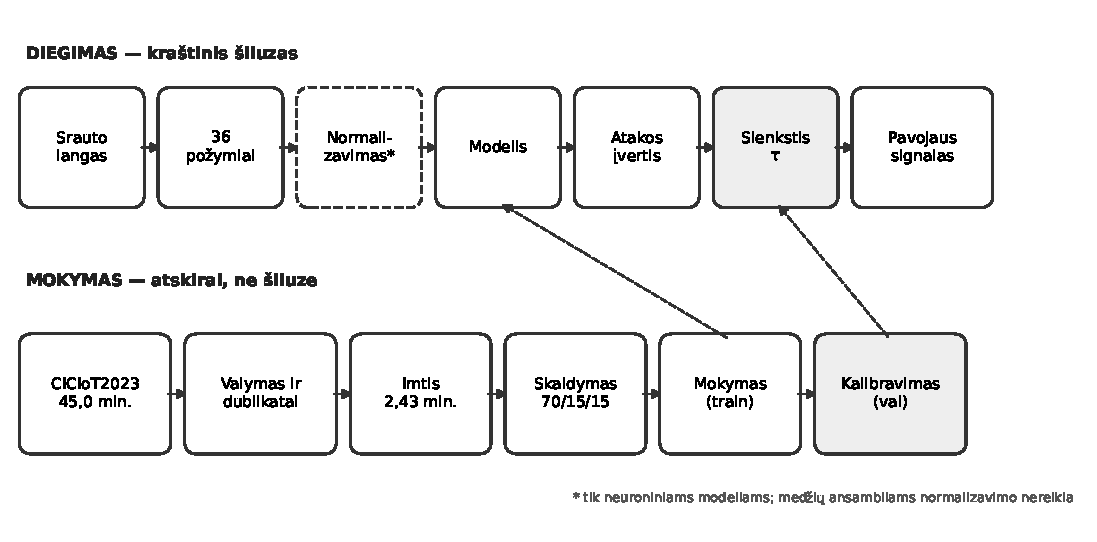
\includegraphics[width=\textwidth]{architektura.pdf}
  \caption{Aptikimo sprendimo architektūra}
  \label{pav:architektura}
\end{figure}

Slenkstis nustatomas iš validacijos aibės, ne iš diegimo srauto. Pagal
stebimą srautą kalibruojama sistema prisitaikytų prie atakos, jei ši
truktų pakankamai ilgai.


\subsection{Duomenų paruošimas}
\label{sec:duomenu_paruosimas}

Iš \num{45019243} rinkinio eilučių pašalinamos nutrūkusios ir turinčios
begalines \texttt{Rate} reikšmes, iš viso \num{1000}. Toliau šalinami
tikslūs dublikatai, ir tik po to sudaroma imtis.

\begin{table}[htbp]
\centering
\caption{Duomenų rinkinys pagal kategorijas: dublikatų dalis, unikalių
         eilučių skaičius ir imtis}
\label{tab:imtis}
\lentele{imtis.tex}
\end{table}

Dublikatai pasiskirstę netolygiai (\ref{tab:imtis} lentelė): potvynio
klasėse jų yra dešimtys procentų, o gerybiniame sraute ir retose atakų
klasėse beveik nėra. Todėl dublikatų šalinimas pats savaime mažina
disbalansą, nes traukiasi gausiausios klasės.

Imtis sudaroma taikant \num{100000} eilučių ribą kiekvienai etiketei;
retos klasės imamos visos. Rezultatas yra \num{2425937} eilutės, arba
5,4~\% valyto rinkinio. Trylikai klasių iš 34 riba neįsijungia, o
mažiausia klasė \texttt{UPLOADING\_ATTACK} turi \num{1196} eilutes.

Kadangi riba taikoma etiketei, kategorijų dydžiai imtyje lieka labai
nevienodi. Disbalansas imtyje yra 84:1; be ribos jis būtų 5764:1.

Prieštaringos etiketės, t.\,y. vienodi požymių vektoriai, pažymėti
skirtingai, paliekamos kaip tikras duomenų dviprasmiškumas. Imtyje jų yra
\num{5114}, arba \num{10435} eilutės (0,43~\%); teorinė tikslumo riba
šioje imtyje yra 99,78~\%.

Skaidymas yra stratifikuotas atsitiktinis 70/15/15: \num{1698155}
eilutės mokymui, po \num{363891} validacijai ir testavimui.
Stratifikuojama pagal 34 etiketes, nes kategorija yra etiketės funkcija,
tad kategorijų proporcijos išlieka savaime. Didžiausias klasės
proporcijos nuokrypis mokymo aibėje siekia 0,0001 procentinio punkto.


\subsection{Požymių atranka}
\label{sec:pozymiai}

Iš 39 leidimo požymių šalinami trys, kurių ryšys su kitais yra tikslus:
\texttt{Variance} (= \texttt{Std}$^2$), \texttt{Tot sum}
(= \texttt{AVG} $\times$ \texttt{Number}) ir \texttt{Tot size}
(= \texttt{AVG}). Visos trys tapatybės
patikrintos darbinėje imtyje, nesutapimų nė vieno iš \num{2425937}.
Lieka 36 požymiai.

Šalinama sąrašu, ne automatiniu filtru. Koreliacijos slenkstis šių porų
nepagautų, nes \texttt{Variance} ir \texttt{Std} Pearson koreliacija
tėra \num{0.737}, nors ryšys tikslus. Mažos dispersijos filtras
pašalintų šešis požymius, kurie daugiau nei 99,5~\% eilučių turi tą
pačią reikšmę, bet rečiausiose klasėse įgyja 7--22 kartus didesnes
vidutines reikšmes, o tos klasės ir lemia macro-F1.

\texttt{Protocol Type} paliekamas, nors atrodo perteklinis šalia
\texttt{TCP}, \texttt{UDP} ir \texttt{ICMP} stulpelių. Sutapimas su
jais yra 69,8--94,4~\%, t.\,y. koreliacija, o ne tapatybė.

Vėliavėlių stulpeliai (\texttt{syn\_flag\_number} ir kiti) nėra
dvejetainiai, tai vėliavėlių dalys lange.


\subsection{Modelių realizacija}
\label{sec:sasaja}

Visi keturi metodai realizuoti su vienoda sąsaja: \texttt{fit},
\texttt{predict}, \texttt{predict\_proba} ir išsaugojimas. Du sąsajos
laukai nurodo, ar modelis prižiūrimas ir ar jam būtinas normalizavimas.

\texttt{predict\_proba} grąžina įvertį, kurio didesnė reikšmė reiškia
didesnę atakos tikimybę. Prižiūrimiems metodams tai tikimybių matrica,
autokoderiui atkūrimo paklaida; bendras yra tik rikiavimas, tad
skaičiuojami PR-AUC ir ROC-AUC.

Normalizavimui naudojamas \texttt{StandardScaler}, pritaikomas tik
mokymo aibei. Skalė išsaugoma kartu su modeliu.

Klasių disbalansas sprendžiamas klasių svoriais; jų santykis mokymo
aibėje yra 83,9. XGBoost atveju naudojamas eilučių svorių masyvas, nes
\texttt{scale\_pos\_weight} daugiaklasėje užduotyje neveikia. Gerybinis
srautas nesintetinamas, nes klaidingų teigiamų analizė turi remtis tikru
srautu.


\subsection{Sprendimo slenkstis}
\label{sec:slenkstis}

Prižiūrimi modeliai grąžina tikimybes, tad sprendimo taškas parenkamas
po mokymo. Prie numatytojo pasirinkimo, kai atsakymu imama labiausiai tikėtina
klasė (lentelėse žymima \texttt{argmax}), klaidingų teigiamų dalis
siekia 21--31~\%, t.\,y. 21--31 kartus viršija
\ref{sec:atakos} skyriuje priimtą biudžetą.

Todėl ataka skelbiama tik tada, kai bendra atakų tikimybė viršija
slenkstį $\tau$. Slenkstis parenkamas kaip mažiausias $\tau$,
tenkinantis klaidingų teigiamų biudžetą, ir renkamas tik validacijos
aibėje; išmatuoti operaciniai taškai pateikiami
\ref{sec:slenkscio_kompromisas} poskyryje.

Biudžeto kaina modeliams nevienoda, ir priežastis yra tikimybių
skiriamoji geba. Random Forest tikimybė yra medžių balsų dalis, todėl
ties vienetu ji grubi, o stiprinimo metodas grąžina tolydžias reikšmes
ir aukštą slenkstį pasiekia tiksliau.

Autokoderiui ši taisyklė netaikoma, nes jis klasių neturi. Jo
operacinis taškas yra atkūrimo paklaidos procentilis iš validacijos
aibės gerybinio srauto. Pasirinktas 99-asis procentilis atitinka tą patį 1~\% biudžetą.


\subsection{Eksperimentų infrastruktūra ir prototipas}
\label{sec:infrastruktura}

Kiekvienas eksperimentas aprašomas konfigūracijos failu, kuris nurodo
modelį, užduoties formuluotę ir hiperparametrus; rezultatas yra viena
eilutė bendrame rezultatų faile, iš kurio generuojamos ataskaitos
lentelės.

Du nepriklausomi pilni perleidimai davė kokybės metrikas, sutampančias
iki $1\cdot10^{-5}$.

\begin{table}[htbp]
\centering
\caption{Veikimo rodikliai: mokymo laikas, inferencijos delsa procesoriumi
         ir modelio dydis}
\label{tab:veikimas}
\lentele{veikimas.tex}
\end{table}

Inferencijos delsa (\ref{tab:veikimas} lentelė) matuojama procesoriumi,
nors mokymui naudotas grafinis spartintuvas, nes kraštinis šliuzas jo
neturi.

Sprendimo veikimui pademonstruoti sukurtas prototipas
(\ref{pav:prototipas} paveikslas): rodomi apdorotų langų ir signalų
skaičiai, klaidingų teigiamų dalis, aptikimo dalis pagal kategorijas ir
inferencijos delsa. Prototipas naudoja
tą patį sprendimo tašką kaip vertinimas ir dirba su validacijos aibe.

\begin{figure}[H]
  \centering
  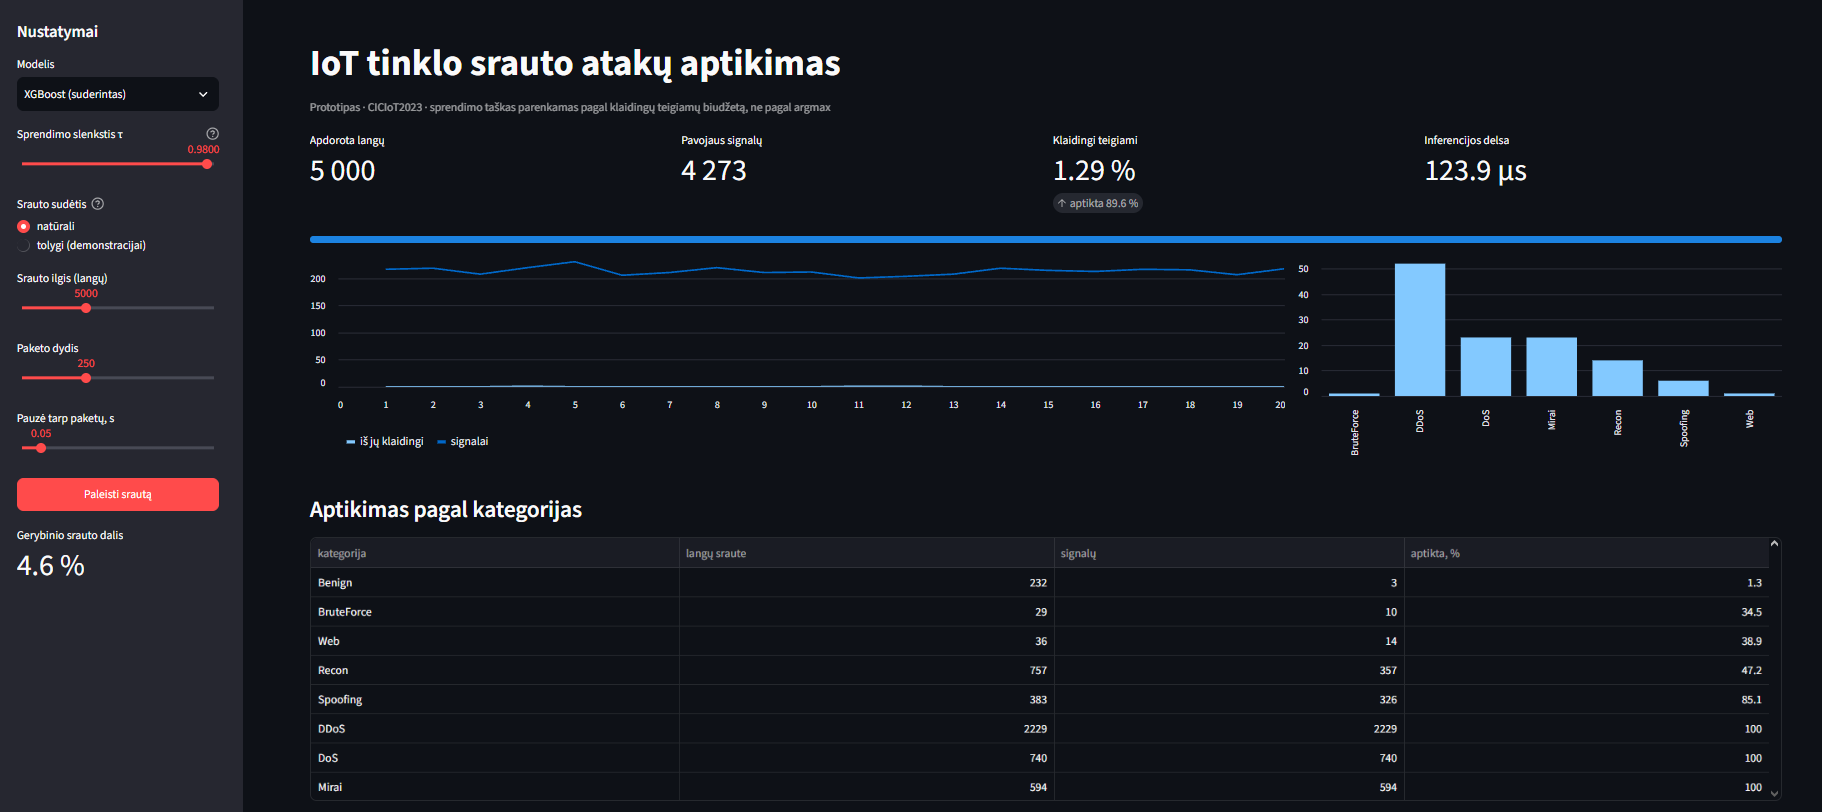
\includegraphics[width=\textwidth]{prototipas.png}
  \caption{Prototipas apdorojant \num{5000} srauto langų. Klaidingų
    teigiamų dalis yra 1,29~\%, aptinkama 89,6~\% atakų. Bendras rodiklis
    slepia skirtumus tarp kategorijų. Potvynio ir Mirai atakos aptinkamos
    visos, o \texttt{BruteForce} ir žiniatinklio atakos aptinkamos mažiau
    nei puse atvejų.}
  \label{pav:prototipas}
\end{figure}

Prototipe išmatuota delsa didesnė nei \ref{tab:veikimas} lentelėje, nes
langai apdorojami po 250. Toks matavimas artimesnis diegimo sąlygoms ir
vis tiek lieka dviem eilėmis žemiau biudžeto.



\section{Eksperimentinis vertinimas}
\label{sec:vertinimas}
% ---------------------------------------------------------------------
%  5 UŽDUOTIS — Eksperimentinis vertinimas
%  REIKALINGA PREAMBULĖJE: xltabular, tabularx, booktabs, siunitx,
%                          graphicx, float, multirow
%  Lentelės ir paveikslai GENERUOJAMI:
%    python -m src.eksperimentai.i_latex --aibe test --priesaga _test
%    python -m src.eksperimentai.klaidos --aibe test
%    python -m src.eksperimentai.slenkstis --taikyti test
%    python -m src.eksperimentai.nematytos
%    python -m src.eksperimentai.patikimumas --su-duomenimis
%    python -m src.eksperimentai.paveikslai
% ---------------------------------------------------------------------

\subsection{Vertinimo protokolas ir operacinis taškas}
\label{sec:vertinimo_protokolas}

Testavimo aibė iki šio skyriaus nebuvo atidaryta nė karto. Visi
sprendimai --- hiperparametrai, ankstyvas stabdymas, požymių sąrašas ir
sprendimo slenkstis --- priimti mokymo ir validacijos aibėse, o testavimo
aibė panaudota vienu prėjimu, iš kurio gauti visi šiame skyriuje
pateikiami pjūviai.

Vertinami keturi modeliai suderintomis konfigūracijomis, po tris
paleidimus su skirtingais pradiniais dydžiais; pateikiamas vidurkis ir
standartinis nuokrypis. Pagrindinė formuluotė --- aštuonios kategorijos;
dvejetainė ir 34 klasių nagrinėjamos atskirai (\ref{sec:formuluotes}
poskyris).

Palyginimas atliekamas ties \textbf{suderintu klaidingų teigiamų
biudžetu}, o ne ties didžiausios tikimybės taisykle. Slenkstis
$\tau$ kiekvienam modeliui parinktas validacijos aibėje kaip mažiausias,
tenkinantis 1~\% biudžetą, ir testavimo aibėje netaikomas iš
naujo: perrinkimas toje pačioje aibėje, kurioje matuojama, būtų
nutekėjimas. Didžiausios tikimybės taškas pateikiamas šalia, nes ties juo
modelių rikiuotė yra kitokia --- tai savarankiškas rezultatas, aptariamas
\ref{sec:slenkscio_kompromisas} poskyryje.

Skirtumas tarp modelių laikomas tikru tik tada, kai jis viršija
paleidimų sklaidą. Formalus statistinis testas neatliekamas: trijų
paleidimų $t$~testas turi pervertintą pirmos rūšies klaidos tikimybę
\cite{dietterich1998tests}.


\subsection{Pagrindiniai rezultatai}
\label{sec:pagrindiniai_rezultatai}

\begin{table}[htbp]
\centering
\caption{Aptikimo kokybė testavimo aibėje.}
\label{tab:rezultatai_test}
\lentele{rezultatai_test.tex}
\end{table}

Ties didžiausios tikimybės tašku geriausią makro-F1 pasiekia
Random~Forest (\num{0.7276}), po jo XGBoost (\num{0.7210}) ir MLP
(\num{0.6346}). Skirtumas tarp dviejų pirmųjų yra \num{0.0066}, o
paleidimų sklaida --- \num{0.0001}, todėl jis nėra atsitiktinis.

Ties klaidingų teigiamų biudžetu rikiuotė apsiverčia: XGBoost pasiekia
makro-F1 \num{0.6626} prie 0,95~\% klaidingų teigiamų, o
Random~Forest --- \num{0.6455} prie 1,02~\%. Priežastis yra
tikimybių skiriamoji geba: Random~Forest tikimybė yra medžių balsų dalis,
todėl ties vienetu ji kinta šuoliais, o XGBoost grąžina tolydžias
reikšmes ir aukštą slenkstį pasiekia tiksliau. Tas pats reiškinys buvo
išmatuotas ir validacijos aibėje, ir su nesuderintomis
hiperparametrų reikšmėmis, todėl tai modelių savybė, o ne vieno matavimo
ypatybė.

Autokoderis makro-F1 skalėje su prižiūrimais modeliais nelyginamas: jis
sprendžia dvejetainį uždavinį, o jo \num{0.2187} gaunamas prie
0,93~\% klaidingų teigiamų --- taško, kurį jis pasiekia pagal
konstrukciją, nes slenkstis yra gerybinio srauto atkūrimo paklaidos
procentilis.

\begin{table}[htbp]
\centering
\caption{Veikimo rodikliai testavimo aibėje: mokymo laikas, gryna
  inferencijos delsa procesoriumi ir modelio dydis diske.}
\label{tab:veikimas_test}
\lentele{veikimas_test.tex}
\end{table}

Inferencijos delsa visiems keturiems modeliams yra
3--30 mikrosekundžių vienam įrašui, t.~y. tris eiles mažesnė už
20--50~ms kraštinio šliuzo biudžetą, nustatytą
\ref{sec:atakos} skyriuje. Ribojantis resursų rodiklis yra ne delsa, o
\textbf{modelio dydis}: suderintas Random~Forest užima 638~MB
diske, o įkeliamas į atmintį --- kelis kartus daugiau, todėl kraštinio
šliuzo klasės įrenginyje, turinčiame 1--8~GB, jis netelpa. XGBoost su
45~MB telpa be išlygų.


\subsection{Klaidų analizė}
\label{sec:klaidu_analize}

Bendras tikslumas visas klaidas skaičiuoja vienodai, nors eksploatacijai
jos kainuoja skirtingai. \ref{tab:klaidu_tipai} lentelėje klaidos
suskirstytos į tris rūšis: klaidingi teigiami (gerybinis srautas
paskelbtas ataka), praleistos atakos ir painiava \emph{tarp atakų}, kai
pavojaus signalas įvyksta, o suklystama tik kategorija.

\begin{table}[htbp]
\centering
\caption{Klaidų pasiskirstymas pagal eksploatacinę kainą.}
\label{tab:klaidu_tipai}
\lentele{klaidu_tipai.tex}
\end{table}

Beveik keturios klaidos iš penkių yra tarp atakų. Iš XGBoost
\num{61651} klaidos \num{39155} sudaro viena pora: \num{33379} DDoS
eilučių priskirtos DoS ir \num{5776} DoS eilučių --- DDoS, t.~y.
63,5~\% visų klaidų. Abi kategorijos kraštiniame šliuze
sukelia tą patį veiksmą, o jas skirianti informacija --- srauto šaltinių
skaičius ir kryptis --- šiame duomenų rinkinio leidime neišreikšta.

Iš to seka, kad tikslumas \num{0.8303} nereiškia, jog modelis praleidžia
kas šeštą ataką: du trečdaliai atotrūkio nuo vieneto yra riba, kurios
turimi požymiai neleidžia nubrėžti, o ne neaptiktos atakos.

\begin{figure}[H]
  \centering
  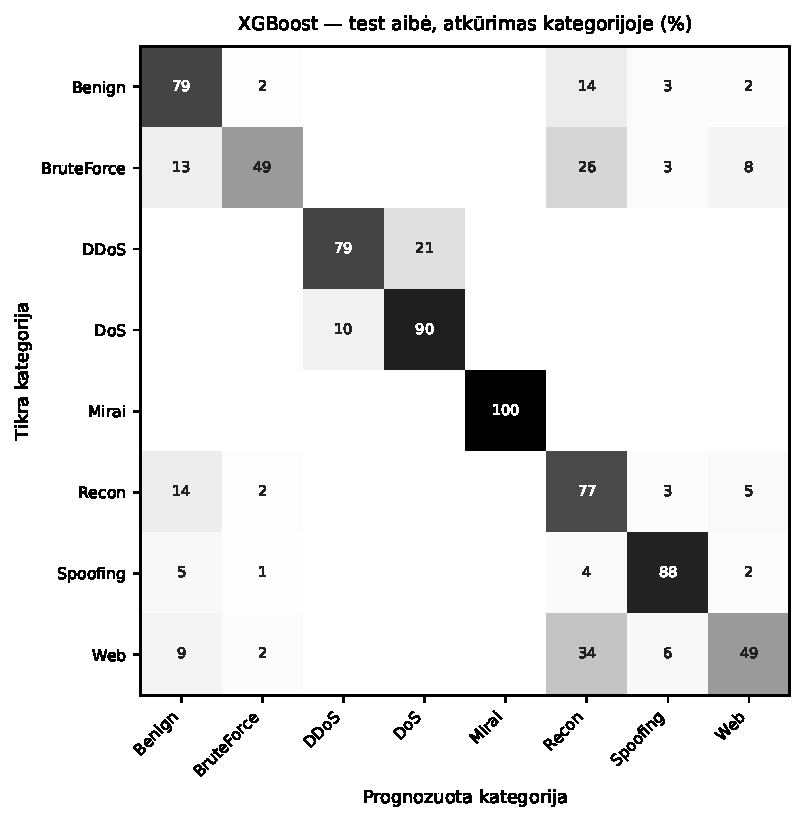
\includegraphics[width=0.82\textwidth]{sumaisymas.pdf}
  \caption{XGBoost sumaišymo matrica testavimo aibėje, normalizuota per
    eilutę. Ryškiausi ne įstrižainės langeliai --- DDoS ir DoS riba bei
    gerybinio srauto ir žvalgybos pora.}
  \label{pav:sumaisymas}
\end{figure}

Antra stambi klaidų grupė turi vardą, numatytą dar
\ref{sec:atakos} skyriuje. Tikras gerybinis srautas, kurį modelis
paskelbia ataka, beveik visas virsta \emph{žvalgyba}: Random~Forest ---
21,2~\% viso gerybinio srauto, XGBoost --- 14,5~\%.
Painiava abipusė: \num{7770} žvalgybos eilučių priskiriamos gerybiniam
srautui, todėl gerybinio srauto tikslumas tesiekia \num{0.543}.

Tai tiesioginė \ref{tab:atakos} lentelėje užfiksuoto apribojimo pasekmė.
Žvalgybos eilutėje ten nurodyta, kad srauto kryptis, trukmė ir unikalių
taikinių skaičius šiame leidime nefiksuojami --- o būtent jie skiria
prievadų skenavimą nuo įprasto jungčių srauto. Teorinėje dalyje įvardytas
požymių trūkumas eksperimente pasirodė kaip konkretus, išmatuojamas klaidų
šablonas.

\begin{table}[htbp]
\centering
\caption{Per-kategorijų rodikliai testavimo aibėje.}
\label{tab:perklase}
\lentele{perklase.tex}
\end{table}

Makro-F1 lygį lemia dvi mažiausios kategorijos. \emph{Web}
($n = \num{3556}$) ir \emph{BruteForce} ($n = \num{1878}$) F1 yra
0,38--0,47 medžių ansambliuose ir 0,21--0,22 MLP,
o \emph{Mirai} --- \num{0.998}. Retose kategorijose didžiausia ir
paleidimų sklaida, todėl pagrindinio rodiklio neapibrėžtumas kyla būtent
iš jų.

MLP klysta kitaip nei medžių ansambliai: jo klaidingi teigiami eina ne į
žvalgybą, o į \emph{Web} ir \emph{BruteForce}, kurių tikslumas tesiekia
0,125--0,137 prie atkūrimo 0,60--0,62. Klasių
svoriai jį verčia retas kategorijas skelbti per dažnai, o medžių
ansambliuose tas pats svertas veikia priešinga kryptimi.


\subsection{Klaidingi teigiami ir slenksčio kompromisas}
\label{sec:slenkscio_kompromisas}

\begin{table}[htbp]
\centering
\caption{Operaciniai taškai testavimo aibėje. $\tau$ parinktas
  validacijos aibėje.}
\label{tab:slenkstis_test}
\lentele{slenkstis_test.tex}
\end{table}

Ties didžiausios tikimybės tašku prižiūrimų modelių klaidingų teigiamų
dalis yra 21--31~\% --- 21--31 kartą daugiau už
\ref{sec:atakos} skyriuje nustatytą biudžetą. Įvedus slenkstį, XGBoost
klaidingi teigiami krenta iki 0,95~\%, o aptikimas išlieka
88,5~\%: klaidingų teigiamų sumažėja daugiau nei
dvidešimt kartų, o makro-F1 --- 8~\%. Modelis nepermokomas;
keičiasi tik sprendimo taisyklė.

\begin{figure}[H]
  \centering
  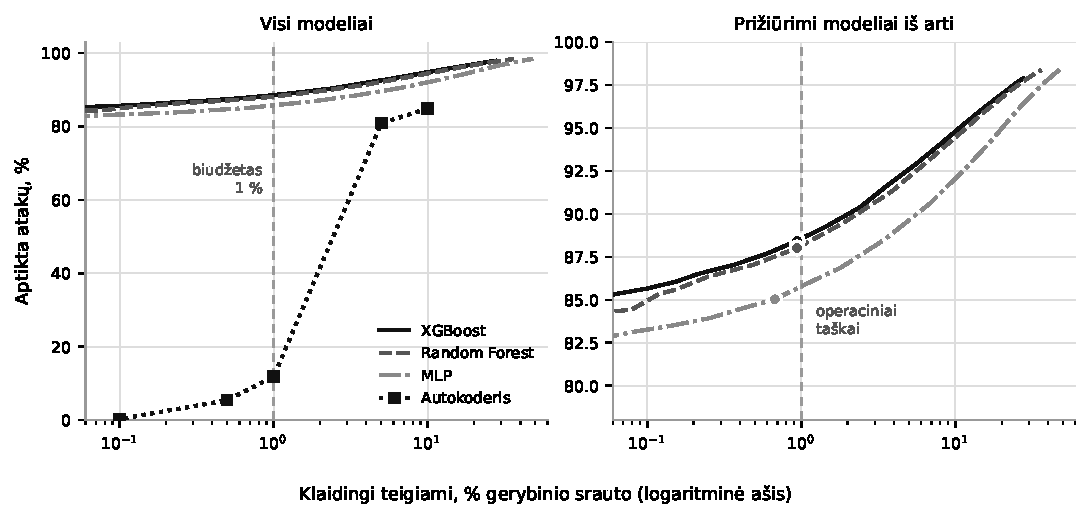
\includegraphics[width=\textwidth]{kreives.pdf}
  \caption{Klaidingų teigiamų ir aptikimo kompromisas validacijos aibėje.
    Kairėje --- visi keturi modeliai; dešinėje priartinti prižiūrimieji su
    pažymėtais operaciniais taškais.}
  \label{pav:kreives}
\end{figure}

Autokoderio kreivė yra kitos rūšies. Tarp 95-ojo ir 99-ojo procentilio
jo aptikimas krenta nuo 80,9~\% iki 11,8~\%, o
prižiūrimi modeliai tame pačiame rėžyje lieka virš 83~\%.
Autokoderis \emph{rikiuoja} gerai --- jo PR-AUC didesnis už atsitiktinio
rikiavimo lygį --- bet reikalaujamo klaidingų teigiamų biudžeto viduje
naudingo aptikimo lygio nepasiekia. Tai stipresnis teiginys nei
konstatavimas, kad jis silpnesnis: jis pasako, kuriame taške ir kodėl.

\begin{figure}[H]
  \centering
  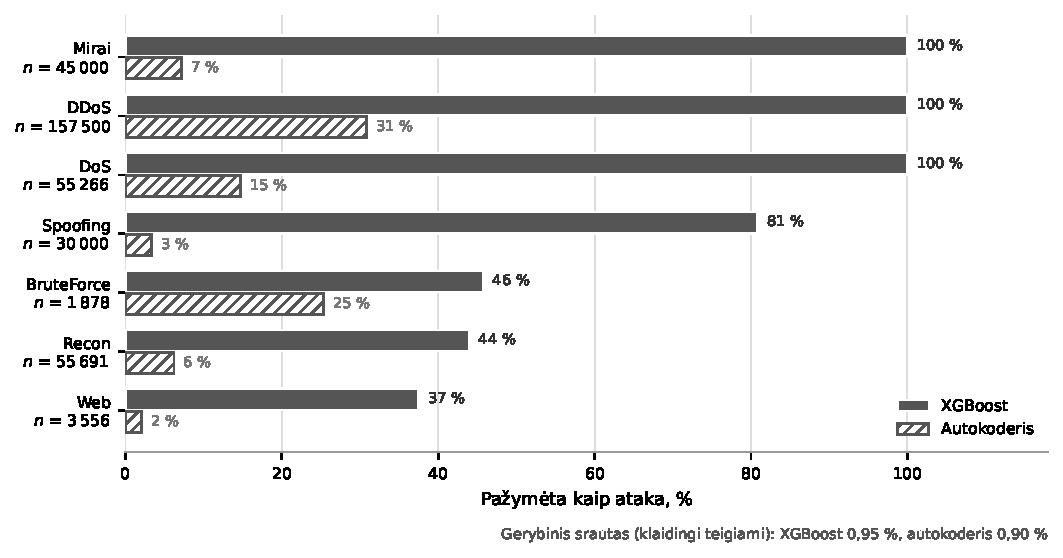
\includegraphics[width=\textwidth]{kategorijos.pdf}
  \caption{Aptikimas pagal kategorijas ties klaidingų teigiamų biudžetu
    testavimo aibėje. Gerybinio srauto eilutės nėra: jai tas pats
    stulpelis reikštų klaidingus teigiamus, ne aptikimą.}
  \label{pav:kategorijos}
\end{figure}

Bendras aptikimo rodiklis yra svertinis vidurkis, kurį lemia gausiausios
kategorijos. Ties tuo pačiu operaciniu tašku DDoS, DoS ir Mirai
aptinkamos 100~\%, o \emph{Recon} --- 43,9~\%,
\emph{Web} --- 37,5~\%. Rėžis per kategorijas yra
37--100~\%, ir prasčiausiai aptinkamos yra kaip tik tos,
kurios saugumo požiūriu svarbios kaip ankstyvas įspėjimas. Klaidingų
teigiamų biudžeto laikymasis perkamas žvalgybos aptikimu.


\subsection{Nematytų atakų klasių testas}
\label{sec:nematytos}

Neprižiūrimo metodo įtraukimas į palyginimą rėmėsi prielaida, kad
nematytoms atakoms reikia modelio, kuris atakų pavyzdžių nemato. Ši
prielaida patikrinta tiesiogiai: prižiūrimas modelis permokytas be
kiekvienos iš trijų klasių, parinktų dar \ref{sec:parinkimas} skyriuje,
ir įvertintas ta pačia testavimo aibe.

Klausiama vieno dalyko --- ar pašalintos klasės eilutės pažymimos kaip
\emph{bet kuri} ataka. Makro-F1 čia netinka: pašalinus
\texttt{DICTIONARYBRUTEFORCE} ištuštėja visa \emph{BruteForce}
kategorija, ir modelis vidurkinamas per septynias klases vietoj aštuonių.
Autokoderis nepermokomas --- jis mokomas tik iš gerybinio srauto, todėl
visos 33 atakų klasės jam ir taip nematytos.

\begin{table}[htbp]
\centering
\caption{Nematytų atakų klasių aptikimas testavimo aibėje.}
\label{tab:nematytos}
\lentele{nematytos.tex}
\end{table}

Prižiūrimas modelis, klasės niekada nematęs, aptinka ją geriau už
neprižiūrimą dviem atvejais iš trijų, o trečiuoju jie lygūs
(24,4~\% prieš 25,4~\%). Prielaida, kad zero-day
atakoms būtinas neprižiūrimas metodas, šiuose duomenyse nepasitvirtina.

Svarbesnis už rikiuotę yra klasės nematymo \emph{kaina}, matoma
sugretinus paskutinius du stulpelius:

\begin{itemize}\itemsep2pt
  \item \texttt{DDOS-SLOWLORIS} --- 0,0 procentinio punkto;
  \item \texttt{RECON-PORTSCAN} --- 1,5 procentinio punkto;
  \item \texttt{DICTIONARYBRUTEFORCE} --- 21,3 procentinio punkto.
\end{itemize}

Skirtumą lemia ne pati klasė, o tai, ar išlieka jos kategorija. Pirmųjų
dviejų kategorijose lieka atitinkamai vienuolika ir keturios giminingos
klasės, ir apibendrinimas joms beveik nemokamas. Trečioji yra vienintelė
savo kategorijos klasė, todėl ją pašalinus prižiūrimas modelis netenka
visos kategorijos, ir aptikimas krenta perpus.

\texttt{DDOS-SLOWLORIS} aptinkama 99,94~\% --- tiek pat, kiek
turint ją mokymo aibėje. Tai neprieštarauja \ref{sec:atakos} skyriuje
nurodytam apribojimui, o iš jo seka: kadangi srauto trukmės požymio
šiame leidime nėra, žemo intensyvumo ataka požymių erdvėje nesiskiria nuo
kitų DDoS klasių. Ji aptinkama patikimai ne todėl, kad modelis ją
atpažįsta, o todėl, kad neatskiria nuo to, kas jau išmokta ---
eksploatacijai signalas įvyksta, bet kategorija nurodoma neteisingai.

Teiginio ribos aiškios: tikrintos trys klasės, kurių kategorijos, išskyrus
vieną, mokymo aibėje liko. Rezultatas galioja naujai tos pačios šeimos
klasei, o ne atakai, nepriklausančiai nė vienai iš aštuonių kategorijų;
tokio atvejo šie duomenys neturi.


\subsection{Dvejetainė ir 34 klasių formuluotės}
\label{sec:formuluotes}

Palyginimui su literatūra geriausias prižiūrimas modelis įvertintas ir
kitomis dviem formuluotėmis, tais pačiais hiperparametrais. Palyginimas
atliekamas ties didžiausios tikimybės tašku, nes tokius skaičius skelbia
cituojami darbai.

\begin{table}[htbp]
\centering
\small
\begin{tabularx}{\textwidth}{@{}>{\raggedright\arraybackslash}X
    >{\centering\arraybackslash}p{2.0cm}>{\centering\arraybackslash}p{2.0cm}
    >{\centering\arraybackslash}p{2.0cm}>{\centering\arraybackslash}p{2.0cm}@{}}
\toprule
\textbf{Formuluotė} & \multicolumn{2}{c}{\textbf{Šis darbas}}
  & \multicolumn{2}{c}{\textbf{\cite{almahaqeri2026gradient}}} \\
\cmidrule(lr){2-3}\cmidrule(l){4-5}
 & tikslumas & makro-F1 & tikslumas & makro-F1 \\
\midrule
Dvejetainė      & 0,9435 & 0,7692 & 0,9961 & 0,9952 \\
8 kategorijos   & 0,8303 & 0,7210 & 0,9959 & 0,8903 \\
34 klasės       & 0,7708 & 0,6464 & 0,9948 & 0,8876 \\
\midrule
\textbf{Rėžis}  & \textbf{0,173} & 0,123 & \textbf{0,001} & 0,108 \\
\bottomrule
\end{tabularx}
\caption{Užduoties detalumo įtaka. Paskutinė eilutė --- skirtumas tarp
  didžiausios ir mažiausios reikšmės stulpelyje.}
\label{tab:formuluotes}
\end{table}

Skiriasi ne tik lygis, bet ir dėsningumo forma. Cituojamame darbe
užduoties detalumas tikslumui beveik neturi įtakos --- rėžis
\num{0.001} --- o makro-F1 krenta \num{0.108}. Šiame darbe makro-F1
kritimas panašus (\num{0.123}), o tikslumo rėžis yra
\num{0.173}, t.~y. daugiau nei šimtą kartų didesnis.

Toks skirtumas yra tai, ko tikėtumeisi, jei mokymo aibėje liktų
pasikartojančių eilučių. Įsiminta eilutė atsakoma teisingai bet kokiu
detalumu --- jai nesvarbu, ar klasių dvi, aštuonios, ar 34. Duomenyse,
iš kurių pašalinta 53,3~\% tikslių dublikatų, modelis privalo
klases tikrai atskirti, todėl kiekvienas detalumo lygis kainuoja.
Sugretinimą riboja ir kiti skirtumai --- 39 požymiai vietoj 46 bei imties
dydis --- todėl teigiama tiek, kad skiriasi dėsningumo forma, o ne tik
lygis.

Didžiausias atotrūkis yra paprasčiausioje užduotyje. Dvejetainėje
formuluotėje viskas priklauso nuo gerybinio srauto ir atakos ribos ---
tos pačios, kurioje glūdi \ref{sec:klaidu_analize} poskyryje aprašyta
žvalgybos painiava, --- o daugiaklasėje makro-F1 tą ribą atskiedžia
lengvai atpažįstamos kategorijos. Dvejetainis tikslumas \num{0.9435}
atrodo aukštas tik todėl, kad gerybinis srautas sudaro
4,1~\% eilučių.

Detalumas kainuoja pagal visas ašis. Perėjus nuo aštuonių kategorijų prie
34 klasių, modelis padidėja nuo 45~MB iki
113~MB, mokymas pailgėja nuo 112~s iki
407~s, delsa auga nuo 29,6 mikrosekundės iki
90,1 mikrosekundės, o makro-F1 krenta. Priežastis struktūrinė:
gradientinio stiprinimo modelis daugiaklasėje užduotyje augina
$n_{\text{medžių}} \times n_{\text{klasių}}$ medžių. Aštuonių kategorijų
detalumas, pasirinktas \ref{sec:di_metodai} skyriuje, taip pasirodo esąs
pagrįstas ir matavimu.


\subsection{Rezultatų patikimumas}
\label{sec:patikimumas}

Prieš rašant skaičius atliktos penkios patikros. Trys jų galioja be
išlygų, dvi davė radinius, kurie yra rezultato dalis.

\textbf{Testavimo aibė neįtakojo nė vieno sprendimo.} Slenkstis $\tau$
testavimo aibėje sutampa su validacijos aibėje parinktu iki paskutinio
skaitmens visiems keturiems modeliams, o kiekviena testavimo aibės eilutė
turi atitinkamą validacijos aibės eilutę --- vadinasi, nė vienas modelis
nebuvo vertintas testavimo aibėje anksčiau nei validacijos.

\textbf{Didžiausias tikslumas neviršija teorinės ribos.} Darbinėje imtyje
0,43~\% eilučių turi prieštaringas etiketes, todėl geriausias
įmanomas klasifikatorius klysta bent tiek; riba yra
99,78~\%, o didžiausias išmatuotas tikslumas ---
\num{0.9436}. Aukštesnis už ribą rezultatas būtų nutekėjimo požymis, ne
pasiekimas.

\textbf{Lentelių skaičiai atkuriami nepriklausomu keliu.} Kokybės
metrikos perskaičiuotos iš išsaugotų sumaišymo matricų ir sugretintos su
eksperimentų failu: didžiausias skirtumas dvylikoje paleidimų ---
$4{,}5 \cdot 10^{-6}$.

\begin{table}[htbp]
\centering
\caption{Operacinio taško perkeliamumas iš validacijos į testavimo aibę.}
\label{tab:patikimumas}
\lentele{patikimumas.tex}
\end{table}

\textbf{Pirmasis radinys --- operacinio taško perkeliamumas.} Klaidingų
teigiamų dalis testavimo aibėje nuo validacijos aibės vertės skiriasi
0,95--1,13 karto, tad taškas persikelia. Tačiau Random~Forest
peržengia biudžetą: 1,02~\% vietoj 1~\%.
Priežastis yra parinkimo taisyklėje --- imamas \emph{mažiausias} $\tau$,
tenkinantis biudžetą, todėl jis pagal konstrukciją atsiduria prie pat
ribos ir atsargos neturi. Eksploatacijai iš to seka konkretus
reikalavimas: slenkstį rinkti su atsarga, pavyzdžiui, ties
80~\% biudžeto.

\textbf{Antrasis radinys --- dedublikavimo ir požymių atrankos tvarka.}
Mokymo ir testavimo aibės nesikerta 39 stulpelių erdvėje, kurioje buvo
šalinami dublikatai. Tačiau 36 požymių erdvėje, kurią mato modelis,
sutampa \num{30} eilučių, t.~y. 0,0082~\% testavimo aibės.
Priežastis --- pašalinti požymiai. Eilutės, kurios skiriasi paskutiniu
slankiojo kablelio bitu vien pašalintame stulpelyje, po požymių atrankos
tampa tapačios. Poveikis rezultatams neviršija \num{0.0082} procentinio
punkto, t.~y. lieka žemiau pateikiamo tikslumo, tačiau iš to seka
bendresnė taisyklė: dedublikavimas ir požymių atranka turi vykti toje
pačioje erdvėje.


\subsection{Apibendrinimas}
\label{sec:vertinimo_apibendrinimas}

Testavimo aibėje išmatuoti visi keturi modeliai trimis paleidimais,
atlikta klaidų analizė, nematytų atakų klasių testas ir palyginimas su
literatūra, o rezultatai patikrinti penkiomis patikromis.

Geriausias sprendimas ties reikalaujamu klaidingų teigiamų biudžetu yra
XGBoost: makro-F1 \num{0.6626}, aptinkama 88,5~\% atakų prie
0,95~\% klaidingų teigiamų, modelio dydis
45~MB, delsa 29,6 mikrosekundės. Dviejose užduoties
vietose rezultatą riboja ne modelis, o duomenys: gerybinio srauto ir
žvalgybos riba bei DoS ir DDoS skirtis, kurioms reikalingų krypties ir
trukmės požymių šiame leidime nėra.

\ref{sec:di_metodai} skyriuje nurodytas realistinis makro-F1 taikinys
0,85--0,90 nepasiektas. Trys išmatuoti veiksniai paaiškina
skirtumą: pašalinti 53,3~\% tikslių dublikatų, 39 požymių
leidimas vietoj 46 ir palyginimas ties klaidingų teigiamų biudžetu, o ne
ties didžiausios tikimybės tašku. Nė vienas iš jų nėra prielaida.


\section{Metodų efektyvumo palyginimas}
\label{sec:palyginimas}
% ---------------------------------------------------------------------
%  6 UŽDUOTIS — DI metodų efektyvumo palyginimas
%  REIKALINGA PREAMBULĖJE: tabularx, booktabs, siunitx, graphicx, float
%  Lentelės ir paveikslai GENERUOJAMI:
%    python -m src.eksperimentai.suvestine
%    python -m src.eksperimentai.pozymiu_svarba
%  Naujų eksperimentų šis skyrius nedaro: visi skaičiai imami iš
%  5 užduoties palikto vieno prėjimo per testavimo aibę.
% ---------------------------------------------------------------------

\subsection{Palyginimo pagrindas}
\label{sec:palyginimo_pagrindas}

\ref{sec:vertinimas} skyrius atsakė, kiek kiekvienas modelis pasiekia.
Šis skyrius atsako, kuris iš jų ir kuriomis sąlygomis tinkamiausias, o
tam reikia ne dar vieno metrikų rinkinio, o kompromisų: kiekvienas
pranašumas kuria nors ašimi perkamas nuolaida kita.

Palyginimas atliekamas ties suderintu klaidingų teigiamų biudžetu.
Priežastis nėra formali: ties didžiausios tikimybės tašku modelių
rikiuotė yra kitokia, o pats tas taškas šiame darbe atmestas, nes duoda
21--31~\% klaidingų teigiamų, t.~y. dvidešimt--trisdešimt
kartų daugiau, nei \ref{sec:atakos} skyriuje nustatytas eksploatacijos
biudžetas. Todėl
palyginimas ties argmax matuotų tašką, kurio sistema niekada nedirbtų.

Suvestinė turi dvi dalis. Trys prižiūrimi modeliai sprendžia aštuonių
kategorijų uždavinį, autokoderis --- dvejetainį, todėl bendro makro-F1
stulpelio visiems keturiems sudaryti negalima. Ši asimetrija numatyta dar
renkantis metodus (\ref{sec:di_metodai} skyrius) ir čia tik pateikiama
matomu pavidalu.

Skirtumai vertinami ta pačia taisykle kaip \ref{sec:vertinimas} skyriuje:
tikru laikomas tik toks, kuris viršija paleidimų sklaidą
\cite{dietterich1998tests}.


\subsection{Suvestinė}
\label{sec:suvestine}

\begin{table}[htbp]
\centering
\caption{Metodų palyginimas ties klaidingų teigiamų biudžetu.}
\label{tab:suvestine}
\lentele{suvestine.tex}
\end{table}

Prižiūrimų modelių rikiuotė ties operaciniu tašku yra XGBoost
(\num{0.663}), Random~Forest (\num{0.646}), MLP (\num{0.595}). Visų trijų
aptikimo lygis panašus --- 85--89~\% --- todėl skirtumą
daro ne tai, kiek atakų randama, o kaip tiksliai jos priskiriamos
kategorijoms ir kokia kaina biudžetas išlaikomas.

Du dalykai lentelėje svarbesni už rikiuotę. Pirma, \textbf{Random~Forest
biudžeto neišlaiko}: jo klaidingų teigiamų dalis testavimo aibėje yra
1,02~\%, nors slenkstis validacijos aibėje buvo parinktas
ties 0,94~\%. Antra, \textbf{modelių dydžiai skiriasi
tūkstantį kartų, o kokybė --- dešimtadaliu}: nuo 0,52~MB iki
638~MB makro-F1 pakyla nuo \num{0.595} iki \num{0.646}.
Būtent šis neproporcingumas, o ne rikiuotė, lemia rekomendaciją.

Autokoderis pateikiamas atskirai ir jo skaičiai su prižiūrimais
nelyginami tiesiogiai. Ties savo operaciniu tašku
(0,93~\% klaidingų teigiamų) jis pažymi kaip ataką
18,6~\% atakų srauto, o geriausiai atpažįstamoje
kategorijoje --- DDoS --- 30,8~\%. Tuo pačiu jo PR-AUC yra
\num{0.996}: rikiavimas geras, sprendimas ties reikalaujamu biudžetu ---
ne.


\subsection{Kompromisai}
\label{sec:kompromisai}

\begin{figure}[H]
  \centering
  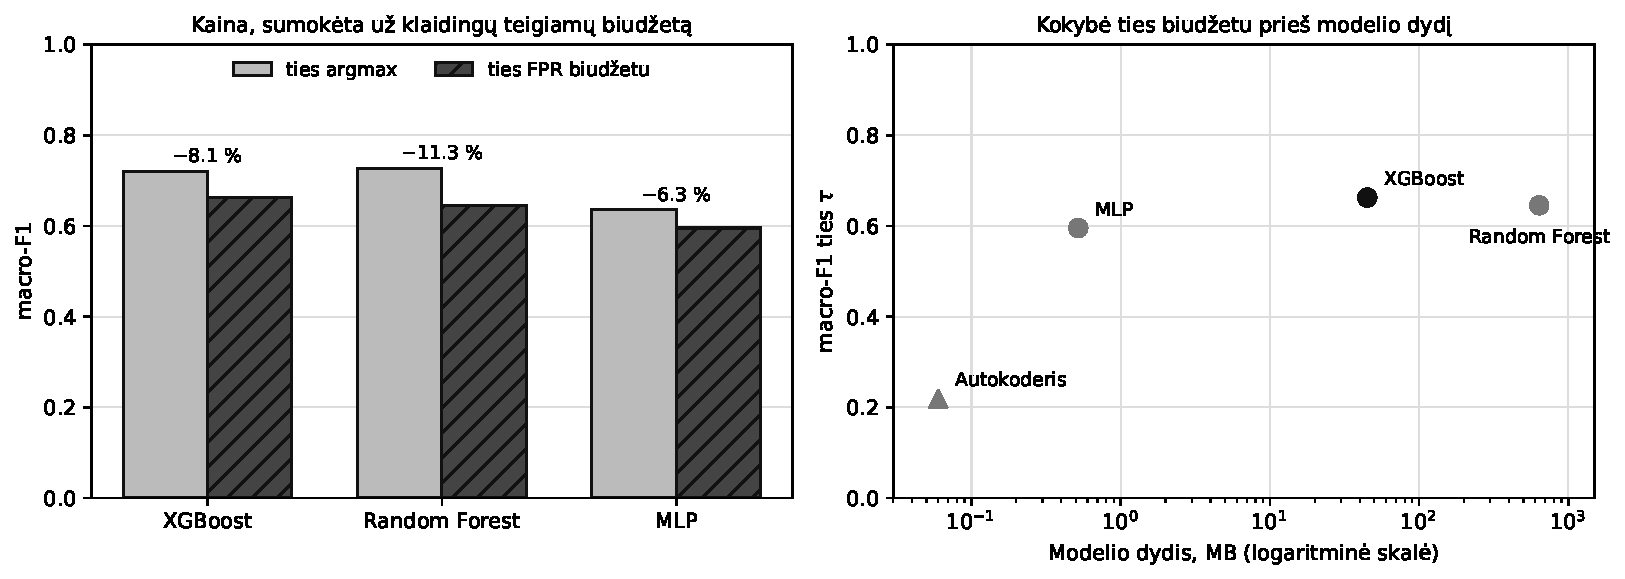
\includegraphics[width=\textwidth]{kompromisai.pdf}
  \caption{Kairėje --- makro-F1 ties didžiausios tikimybės tašku ir ties
    klaidingų teigiamų biudžetu; skaičius virš stulpelių rodo santykinį
    kritimą. Dešinėje --- kokybė ties biudžetu prieš modelio dydį
    logaritmine skale.}
  \label{pav:kompromisai}
\end{figure}

\textbf{Kokybė prieš klaidingus teigiamus.} Biudžeto įvedimas kainuoja
visiems trims modeliams, bet nevienodai: XGBoost netenka
8,1~\% makro-F1, Random~Forest ---
11,3~\%, MLP --- 6,3~\%. Skirtumas
nedidelis absoliučiais dydžiais, bet jo pakanka rikiuotei apversti: ties
argmax pirmauja Random~Forest (\num{0.727} prieš \num{0.721}), ties
biudžetu --- XGBoost (\num{0.663} prieš \num{0.646}).

Priežastis yra tikimybių skiriamoji geba. Random~Forest tikimybė yra
medžių balsų dalis, todėl ties vienetu ji kinta šuoliais, o aukštas
slenkstis reikalauja būtent ten smulkios skalės; XGBoost grąžina
tolydžias reikšmes. Šis reiškinys išmatuotas trimis nepriklausomomis
sąlygomis --- validacijos aibėje, testavimo aibėje ir su nesuderintomis
hiperparametrų reikšmėmis --- todėl laikytinas metodų savybe, o ne vieno
matavimo ypatybe.

Iš to seka bendresnis metodinis teiginys: \emph{palyginimas ties
didžiausios tikimybės tašku ir palyginimas ties klaidingų teigiamų
biudžetu gali duoti skirtingą nugalėtoją}. Darbuose, kur skelbiamas tik
argmax rezultatas, šis skirtumas lieka nematomas.

\textbf{Kokybė prieš resursus.} Ši ašis skiria modelius stipriau nei
kokybė. Random~Forest yra 14 kartų didesnis už XGBoost
(638~MB prieš 45~MB) ir ties operaciniu tašku
prastesnis --- vadinasi, jis nepralaimi kompromise, o yra tiesiog
nurungtas: nė pagal vieną iš keturių atrankos kriterijų jis nėra
geresnis. Praktinė riba dar griežtesnė, nei rodo skaičius diske: modelis
į atmintį įkeliamas kelis kartus didesnis, todėl 1--8~GB
turinčiame kraštinio šliuzo įrenginyje netelpa iš principo.

Tikras kompromisas yra tarp XGBoost ir MLP. MLP yra
86 kartus mažesnis (0,52~MB) ir dešimt kartų
greitesnis, o kainuoja \num{0.068} makro-F1, t.~y.
10~\% santykinio kokybės. Įrenginiams, kuriems 45~MB
per daug --- mikrovaldiklių klasei, apie kurią kalba
\cite{mazinani2026constrained} --- tai reali alternatyva, o ne
nusileidimas.

Delsa nė vieno modelio neriboja: 3--30 mikrosekundžių
vienam įrašui yra trys eilės atsargos iki 20--50~ms
šliuzo biudžeto. Tai patvirtina \ref{sec:di_metodai} skyriuje iš
literatūros perimtą teiginį savais matavimais ir kartu paaiškina, kodėl
resursų kriterijų šiame uždavinyje realiai atstoja modelio dydis.

\textbf{Užduoties detalumas.} Detalumas yra ketvirtoji ašis, ir ji
vienintelė neduoda jokio kompromiso. Perėjus nuo aštuonių kategorijų prie
34 klasių, modelis padidėja 2,5 karto, mokymas pailgėja
3,6 karto, delsa auga 3,0 karto, o makro-F1 krenta
nuo \num{0.721} iki \num{0.646}. Smulkesnis detalumas kainuoja visomis
ašimis ir negrąžina nieko, todėl aštuonių kategorijų formuluotė yra ne
kompromisas, o geresnis pasirinkimas.

\textbf{Prižiūrimas prieš neprižiūrimą.} Autokoderio ir prižiūrimų
modelių skirtumas ties tuo pačiu klaidingų teigiamų biudžetu yra ne
laipsniškas: 18,6~\% prieš 85--89~\%
aptikimo. Kartu jo PR-AUC (\num{0.996}) rodo, kad anomalijos įvertis
atakas nuo gerybinio srauto \emph{rikiuoja} gerai. Abu teiginiai teisingi
ir neprieštarauja: rikiavimo kokybė virsta sprendimo kokybe tik tada, kai
egzistuoja slenkstis, ties kuriuo abu reikalavimai tenkinami vienu metu,
o gerybinio srauto atkūrimo paklaidos pasiskirstyme tokio taško nėra.


\subsection{Prognozės ir matavimas}
\label{sec:prognozes}

Metodai buvo parinkti \ref{sec:parinkimas} skyriuje pagal svertinę
sprendimų matricą, prieš atliekant eksperimentus. Prižiūrimų modelių
balai buvo XGBoost \num{4.70}, Random~Forest \num{3.55}, MLP \num{3.25};
matavimas ties operaciniu tašku davė \num{0.663}, \num{0.646} ir
\num{0.595} --- \textbf{tą pačią tvarką}. Tai prognozė, pateikta prieš
eksperimentą ir pasitvirtinusi, o ne paaiškinimas po fakto.

Sutapimas turi dvi išlygas, ir abi vertingesnės už patį sutapimą.

Pirma, \textbf{tvarka sutampa tik ties operaciniu tašku}. Ties argmax
matavimas duoda kitą pirmąją vietą, nors matrica yra ta pati. Vadinasi,
sprendimų matrica prognozavo ne šiaip metodo kokybę, o kokybę
sąlygomis, kurias pati matrica ir aprašo --- klaidingiems teigiamiems ten
skirta 30~\% svorio.

Antra, \textbf{vienas matricos įvertis buvo klaidingas}. Random~Forest už
resursus gavo 4 balus iš 5, o realiai jo modelis yra
638~MB ir į kraštinio šliuzo įrenginį netelpa. Klaida
sisteminė, ne atsitiktinė: balas remėsi algoritmo savybėmis, o modelio
dydis priklauso nuo mokymo aibės dydžio, kurio balų skalė neapima. Tas
pats pasirodė ir derinimo etape --- 400\,000 eilučių imtyje išmatuotas
196~MB dydis pilnoje aibėje virto 638~MB.

Lieka ir vienas nepatikrintas matricos teiginys: sprendimų medis surinko
\num{3.80} balo, t.~y. daugiau nei Random~Forest, bet į eksperimentą
nepateko, nes ketvertas buvo sudarytas ne vien pagal balus. Ar pigiausias
ir savaime paaiškinamas prižiūrimas metodas ties klaidingų teigiamų
biudžetu prilygtų gradientiniam stiprinimui, šis darbas atsakymo neturi.


\subsection{Nematytos atakos: hipotezės verdiktas}
\label{sec:zero_day}

Autokoderis į palyginimą įtrauktas ne dėl balo --- matricoje jis
pralaimėjo Isolation~Forest (\num{2.95} prieš \num{3.50}) --- o dėl
funkcinio reikalavimo aptikti atakas, kurių pavyzdžių mokymo aibėje
nebuvo. Toks pagrindimas yra tikrinamas teiginys, ir
\ref{sec:nematytos} poskyryje jis patikrintas.

Rezultatas neigiamas: prižiūrimas modelis, klasės niekada nematęs,
aptinka ją geriau dviem atvejais iš trijų, o trečiuoju abu metodai
lygūs. Palyginimui tai reiškia dvi išvadas.

Pirma, \textbf{neprižiūrimas metodas ketverte savo vietos nepateisino}.
Jis pralaimi ir pagrindinį uždavinį, ir tą, kuriam buvo įtrauktas. Iš
matricos seka, kad ketvirtoji vieta būtų buvusi naudingesnė
Isolation~Forest arba antram prižiūrimam metodui.

Antra --- ir tai svarbiau --- \textbf{apibendrinimo geba priklauso ne nuo
paradigmos, o nuo to, ar mokymo aibėje lieka gimininga klasė}. Kai
pašalinama viena klasė, o jos kategorija išlieka, prižiūrimo modelio
aptikimas nukrenta 0,0--1,5 procentinio punkto; kai
ištuštėja visa kategorija --- 21,3 punkto. Zero-day
klausimas todėl yra ne „prižiūrimas ar neprižiūrimas“, o „ar nauja ataka
patenka į jau žinomą šeimą“.

Teiginio ribos nurodytos \ref{sec:nematytos} poskyryje ir galioja
nepakitusios: tikrintos trys klasės, ir nė viena jų nebuvo naujo tipo
ataka, nepriklausanti jokiai iš aštuonių kategorijų.


\subsection{Kuo modelis remiasi}
\label{sec:pozymiu_svarba}

Interpretuojamumui atrankoje skirta 15~\% svorio, ir šis
kriterijus yra vienintelis, kurio prižiūrimų modelių palyginimas iki šiol
nelietė. Medžių ansamblis leidžia jį įvertinti be papildomo skaičiavimo:
vidutinis informacijos prieaugis apskaičiuojamas iš paties modelio, o ne
iš duomenų.

\begin{table}[htbp]
\centering
\caption{Dešimt daugiausiai informacijos prieaugio duodančių požymių.}
\label{tab:pozymiai}
\lentele{pozymiai.tex}
\end{table}

Pasiskirstymas labai netolygus: vienas požymis --- paketų skaičius
lange --- surenka 62,3~\% viso prieaugio, o penki
pirmieji kartu 80,4~\%. Tai atitinka imties sudėtį: DDoS,
DoS ir Mirai kategorijos kartu sudaro 70,8~\% eilučių, o
nuo gerybinio srauto jas skiria būtent intensyvumas. Tos pačios trys
kategorijos ties operaciniu tašku aptinkamos 100~\%. Kartu iš to seka
apribojimas --- modelis, kurio sprendimą dviem trečdaliais lemia vienas
intensyvumo požymis, žemo intensyvumo atakoms turi mažai atramos, ir
\ref{sec:nematytos} poskyryje aprašytas \texttt{DDOS-SLOWLORIS} atvejis
yra tiesioginė to iliustracija.

Antrą vietą užima protokolo kodas (6,0~\%). Tai
verta atskiro sakinio: rengiant požymių modulį šis stulpelis atrodė
perteklinis, nes rinkinyje jau yra atskiri TCP, UDP ir ICMP požymiai, ir
buvo tikrinamas kaip kandidatas šalinti. Patikra parodė, kad sutapimas
yra 70--94~\%, t.~y. koreliacija, o ne tapatybė, ir
stulpelis buvo paliktas. Svarbos lentelė šį sprendimą patvirtina
matavimu.

Šeši sąmoningai palikti mažos dispersijos požymiai kartu surenka
1,9~\% prieaugio. Jie naudojami visi, tad automatinis
filtras būtų pašalinęs informaciją, o ne triukšmą, tačiau įnašas mažas,
ir tai pasakytina taip pat aiškiai, kaip ir jų palikimo pagrindimas.

Metodo riba akivaizdi: informacijos prieaugis nerodo krypties --- jis
pasako, kuo modelis remiasi, o ne kokia požymio reikšmė reiškia ataką.
Sprendimų paaiškinimui analitikui to nepakanka, ir čia reikėtų
\cite{mohale2025xai} aprašytų priemonių, kurių skaičiavimo kaina yra
atskiro darbo dydžio. MLP ir autokoderis tokio pjūvio be papildomų
priemonių neduoda visai --- tai ir yra praktinė interpretuojamumo
kriterijaus išraiška.


\subsection{Rekomendacija}
\label{sec:rekomendacija}

Vieno atsakymo nėra, nes skiriasi diegimo sąlygos. Iš išmatuotų dydžių
seka keturios rekomendacijos.

\textbf{Kraštinio šliuzo įrenginiui, laikantis 1~\%
klaidingų teigiamų biudžeto, tinkamiausias yra XGBoost su sprendimo
slenksčiu.} Jis pasiekia makro-F1 \num{0.663}, aptinka
88,5~\% atakų prie 0,95~\% klaidingų
teigiamų, užima 45~MB ir vienam įrašui sunaudoja
29,6 mikrosekundės. Slenkstis turi būti parenkamas su
atsarga --- ties maždaug 80~\% biudžeto --- nes ties pačiu
kraštu parinktas taškas į naują duomenų aibę persikelia be atsargos, kaip
parodė \ref{sec:patikimumas} poskyrio patikra.

\textbf{Griežtai ribotos atminties įrenginiui tinka MLP.} Jis kainuoja
10~\% makro-F1, bet yra 86 kartus mažesnis ir
biudžeto laikosi patikimiausiai iš visų (0,64~\%).
Alternatyva --- mažesnė gradientinio stiprinimo konfigūracija: derinimo
paieškoje 200 medžių variantas atsiliko mažiau nei
1~\% ir buvo 7,4~MB, tačiau šis dydis matuotas
imtyje, o pilnoje mokymo aibėje jis paauga maždaug pusantro karto.

\textbf{Random~Forest šiam uždaviniui nerekomenduojamas.} Jis ties
operaciniu tašku prastesnis už XGBoost, vienintelis peržengia klaidingų
teigiamų biudžetą ir yra 14 kartų didesnis. Jo vertė šiame darbe --- ne
kaip sprendimo, o kaip atskaitos lygio, ties kuriuo matuojamas
gradientinio stiprinimo prieaugis.

\textbf{Autokoderis kaip vienintelis aptikimo metodas netinka.} Ties
reikalaujamu biudžetu jis aptinka mažiau nei penktadalį atakų srauto ir
nematytoms klasėms neaplenkia prižiūrimo modelio. Kaip papildoma
pakopa --- signalų rikiavimui arba antram vertinimui šalia prižiūrimo
modelio --- jis lieka svarstytinas, nes jo PR-AUC aukštas, o mokymas
trunka sekundes.

Rekomendacijų ribos nurodytinos kartu su jomis. Visi skaičiai gauti
viename duomenų rinkinyje, o kryžminis perkėlimas tarp rinkinių
literatūroje smarkiai krenta \cite{eren2026drift}, todėl rikiuotė
galioja šio pobūdžio srautui, o ne bet kuriam IoT tinklui. Zero-day
teiginys galioja naujai tos pačios šeimos klasei. Ir dvi svarbiausios
klaidų rūšys --- gerybinio srauto painiava su žvalgyba bei DoS ir DDoS
riba --- yra ne modelio, o duomenų savybė: joms atskirti reikalingų
krypties ir trukmės požymių šiame rinkinio leidime nėra, todėl jokia
metodo pakaita jų nepašalintų.


\section{Išvados}
% ---------------------------------------------------------------------
%  IŠVADOS — dvi pastraipos.
%  Skaičiai čia NEPERRAŠOMI ranka iš atminties — visi jau yra
%  atitinkamų skyrių lentelėse.
%  2026-09-15: sutrauktos iš šešių punktų (po vieną kiekvienam
%  uždaviniui) į dvi pastraipas vadovo nurodymu. Ankstesnė redakcija —
%  git istorijoje.
% ---------------------------------------------------------------------

Darbo tikslas buvo sukurti ir eksperimentiškai įvertinti dirbtiniu
intelektu pagrįstą IoT tinklo kibernetinių atakų aptikimo sprendimą.
Tikslas pasiektas. Iš 18 apžvelgtų metodų dviem pakopomis parinkti
keturi, sukurta visa grandinė nuo žalio srauto iki pavojaus signalo ir
įvertinta nepriklausoma testavimo aibe. Geriausias variantas ties
reikalaujamu 1~\% klaidingų teigiamų biudžetu pasiekia macro-F1
\num{0.6626} prie 0,95~\% klaidingų teigiamų, aptinka 88,5~\% atakų
srauto, telpa į 45~MB ir vienam įrašui sunaudoja apie 30 mikrosekundžių,
t.~y. tris eiles mažiau, nei leidžia kraštinio šliuzo biudžetas.

Ribojantis veiksnys buvo ne metodai, o duomenų struktūra. Keturi iš
aštuonių metodų atmetimų kilo iš to, kad rinkinyje nėra nei laiko eilės,
nei srauto krypties, nei šaltinio identifikatorių, o bendras tikslumas
šiam uždaviniui netinka, nes 78,7~\% klaidų yra painiava tarp pačių
atakų. Du rezultatai galioja plačiau už šį rinkinį. Nugalėtojas
priklauso nuo sprendimo taško, nes ties didžiausios tikimybės tašku
pirmauja Random~Forest, o ties biudžetu, kuriuo sistema realiai dirbtų,
XGBoost; darbuose, skelbiančiuose tik pirmąjį skaičių, rikiuotė gali
būti kita. Paneigta ir darbo prielaida, kad nematytoms atakoms būtinas
neprižiūrimas metodas, nes apibendrinimo geba priklauso ne nuo
paradigmos, o nuo to, ar mokymo aibėje lieka gimininga klasė.


% ─── Literatūra ──────────────────────────────────────────────────────
\newpage
\printbibliography[heading=bibintoc,title={Literatūros sąrašas}]

\end{document}
